\documentclass[12pt,a4paper]{scrartcl}
\usepackage{geometry}
\usepackage[ngerman]{babel}
\usepackage[T1]{fontenc}
\usepackage{slashbox}
\usepackage{verbatim} %mehrzeilige Kommentare
\usepackage{url}
\usepackage[bottom,hang]{footmisc}
\usepackage[onehalfspacing]{setspace}
\usepackage{hyperref}
%\usepackage{bibgerm}
%\usepackage{natbib}
\usepackage{blindtext}
\usepackage[utf8]{inputenc} %ä,ö,ü
\usepackage{amsmath} %Mathematischer Formelsatz
\usepackage{amsfonts} %Mathesymbole
\usepackage{amssymb} %Mathesymbole
\usepackage{setspace}
\usepackage{geometry}
\usepackage{tabularx, calc} %Tabellen
%\usepackage{acronym} %Abkürzungsverzeichnis
\usepackage{color} % Farbe
%\usepackage{titlesec}
\usepackage{graphicx} %Graphiken einfügen
\usepackage[automark, headsepline, footsepline, ilines]{scrpage2} %Kopf- und Fußzeilen
\usepackage{multirow} %Tabelle: mehrere Spalten vereinigen
\usepackage{calc} %Rechnungen
%\usepackage{booktabs} %Verbesserung der Tabellenqualität
\usepackage{tabularx, calc} %Tabellen
\usepackage{longtable} %Tabelle über mehrere Seiten
\usepackage{textcomp} %Sonderzeichen
\usepackage{lmodern} %modernisierte Schriftart
\usepackage{booktabs}
\usepackage{multirow}

\usepackage{ragged2e} 

\deffootnote{1.7em}{2.7em}{{\scriptsize\thefootnotemark~~}} 
\addtokomafont{footnote}{\RaggedRight}
%\usepackage{subfigure}
%\usepackage[square]{natbib} %Literaturverzeichnis für naturwissenschaftliche Arbeiten
%\usepackage{wolke} %Abbildungsunterschrift und Tabellenüberschrift mit Kapitelzahl z.B. Abb.: 1.1
%\usepackage{picinpar} %Bild im Text
%\usepackage{picins} %Bild im Text
%\usepackage{caption} %Abbildungs- und Tabellenbeschriftung
%\usepackage{array} %Matheumgebung ähnlich tabular
%\usepackage{dcolumn} %tabelle:kommata untereinander
\titlehead{
\includegraphics[width=5cm]{euletext.png} \hfill 
\includegraphics[width=6cm]{semvox2.png} }
%\titlehead{
\includegraphics[width=7cm]{euletext.png} \hfill}
 %Titelkopf
\title{$\,$\\  Disambiguierungsstrategien in Dialogsystemen}
\rohead{\leftmark}\cohead{} %Kopfzeile: Kapitelüberschrift rechts, nicht mitte
\setlength{\parindent}{0pt} %ohne Einrückung
%\captionsetup{font={footnotesize,bf}} %Abbildungs-und Tabellenbeschriftung klein und fett
\date{}
\setlength{\headsep}{1,25cm} %Abstand zwischen Kopfzeile und Text
%\titlespacing{\section}{0pt}{*1}{1.3cm} 
\author{}
\linespread{1,5} %Zeilenabstand
\clubpenalty10000 % Hurenkinder und Schusterjungen verhindern
\widowpenalty10000 % Hurenkinder und Schusterjungen verhindern
\displaywidowpenalty=10000 % Hurenkinder und Schusterjungen verhindern
\newenvironment{myitemize}{\begin{itemize}\itemsep -2pt}{\end{itemize}}
\pagestyle{scrheadings}
%\setlength{\heavyrulewidth}{1pt} %Tabularx: Dicke der Linien
%\setcounter{tocdepth}{5} %Tiefe des Inhaltsverzeichnisse: 4: section, subsection, subsubsection + paragraph 								im Inhaltsvereichnis
%\setcounter{secnumdepth}{5} %bis zu welcher Schachtelungstiefe erfolgt die Nummerierung des 												Inhaltsverzeichnisses 4: bis paragraph
%\setlength{\tabcolsep}{8pt}
%  \renewcommand\appendix{\par 
%    \setcounter{section}{0}
%    \setcounter{subsection}{0} 
%    \renewcommand\thesection{\Alph{section}}		%alphabetische Nummerierung der Überschriften im Anhang
%    \renewcommand\thefigure{\Alph{section}\arabic{figure}}} %Nummerierung der Abbildungen im Anhang
%	\renewcommand{\arraystretch}{1,5}    
    
\begin{document}
\pdfoutput=1
\pagenumbering{Roman}

\maketitle
\sffamily
\begin{center}
\huge
\textbf{Bachelorarbeit}\\
\vfill
\LARGE
Fachrichtung Computerlinguistik\\
\vfill
\normalsize
vorgelegt von\\
\Large
\textbf{Lena Enzweiler}\\
\vfill


\normalsize
Saarbrücken,
\today

\end{center}

\thispagestyle{empty}
\rmfamily
\cleardoublepage
$\,$\\
\vfill
Meine Bachelorarbeit entstand im Zeitraum vom Juli 2014 bis Oktober 2014 bei SemVox GmbH unter der Leitung von Prof. Dietrich Klakow und der Betreuung von Pia Kuznik.


\cleardoublepage

\tableofcontents
\cleardoublepage

\addcontentsline{toc}{section}{Abbildungsverzeichnis}
\listoffigures
\cleardoublepage

\addcontentsline{toc}{section}{Tabellenverzeichnis}
\listoftables
\cleardoublepage
\markboth{Abkürzungsverzeichnis}{Abkürzungsverzeichnis}
\addcontentsline{toc}{section}{Abkürzungsverzeichnis}
\section*{Abkürzungsverzeichnis}  

\cleardoublepage

\pagenumbering{arabic}

\renewcommand{\abstractname}{Abstract}
\markboth{Abstract}{abstract}
\subsection*{\centering {Abstract}}  
\begin{abstract}
Die vorliegende Arbeit beschäftigt sich mit der Frage, welche Disambiguierungsstrategien in Sprachdialogsystemen für Benutzer bei hoher kognitiver Belastung am geeignetsten sind. Man fokussiert sich dabei auf Sprachdialogsysteme, welche speziell für die Bedienung während der Autofahrt konzipiert werden. Um der Frage der besten Disambiguierungsstrategie nachzugehen, werden in einem Wizard-of-Oz-Experiment Fahrszenarien simuliert, bei denen die Versuchspersonen mit einem Dialogsystem sprachlich interagieren. Dabei werden ambige Eingaben des Benutzers simuliert worauf das System mit Disambiguierungsstrategien in Form von Nachfragen reagiert, welche eine entsprechende Benutzerreaktion verlangen. Anhand der Versuchsergebnisse wird analysiert, welche Strategien für den Benutzer am einfachsten und effektivsten waren. Insgesamt werden drei Disambiguierungsstrategien verfolgt. Aggregierte Auswahl ohne Pause, aggregierte Auswahl mit Pause, sowie die sequentielle Auswahl. 
\end{abstract}
\newpage
\section{Einleitung}

Dialogsysteme für das Auto müssen so gestaltet werden, dass sie den Fahrer so wenig wie möglich vom Fahren ablenken und ihm so gut wie möglich assistieren. Die Herausforderung für einen Dialog Designer besteht daher darin, Sprachäußerungen so raffiniert zu gestalten, dass dem Benutzer zum Einen alle relevanten Informationen in verständlicher Weise geliefert werden und zum Anderen, dass der Benutzer darauf möglichst einfach antworten und seine Anfragen und Wünsche effizient übermitteln kann. Die Funktionsweise eines Dialogsystems hängt von mehreren Komponenten ab, welche anhand der in Abbildung \ref{odps3} dargestellten Funktionsweise der ODP S3 Plattform der SemVox GmbH\footnote{\label{foot:odps3}\url{http://semvox.de}} kurz erläutert werden. Die ODP S3 Plattform ermöglichst die Umsetzung komplexer Sprachdialoge.  
Zunächst müssen die Spracheingaben des Benutzers zu semantischen Objekten verarbeitet werden. Dabei wird zunächst die Spracheingabe auf eine Grammatik abgeglichen, welche alle möglichen Spracheingaben des Benutzers abfängt und semantischen Objekten zuweist. Diese werden dann von einem Backend-Server verarbeitet, woraufhin eine passende Sprachausgabe ausgelöst wird. 
\begin{figure}[htbp]
\begin{center}
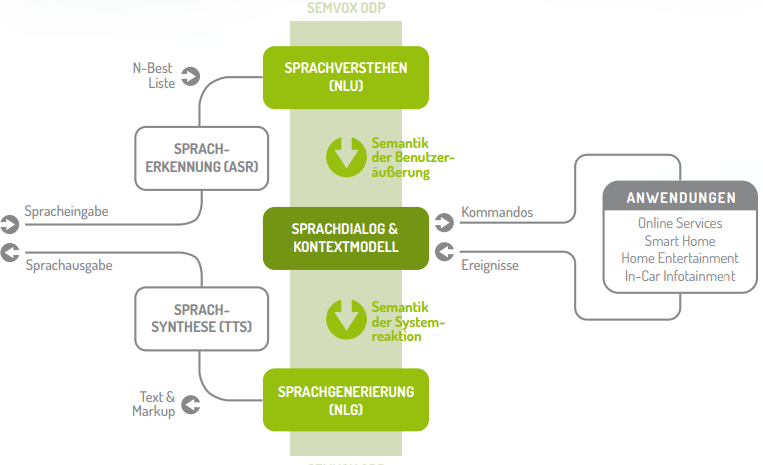
\includegraphics[width=12cm]{odps3.png}
\caption{Funktionsweise der ODP-S3 Platform}
\label{odps3}
\end{center}
\end{figure}
In dieser Arbeit konzentriert man sich allein auf die Sprachgenerierung. Ein komplexer Dialog zwischen System und Benutzer führt häufig dazu, dass der Benutzer eine Eingabe macht, die das System nicht eindeutig zuordnen kann und mehrere Optionen für die Ausführung der vom Benutzer geäußerten Eingabe bestehen. Es muss an dieser Stelle vom System eine Rückfrage beim Benutzer erfolgen, sodass dieser seine vorherige Eingabe eindeutig übermitteln kann. Wenn der Benutzer zum Beispiel den Wunsch äußert einen Kontakt aus dem im System gespeicherten Adressbuch anzurufen, es allerdings zwei Kontakte mit diesem Namen gibt, muss das System eine Rückfrage stellen, um zu ermitteln, welcher dieser beiden Kontakte gemeint ist. Der Dialog Designer spricht in diesem Fall von Disambiguierung.  Es wird in der vorliegenden Arbeit der Frage nachgegangen wie man konkret die Sprachausgabe einer solchen Disambiguierung innerhalb eines Dialogsystems, das speziell für das Auto konzipiert wurde, gestaltet. Dabei werden drei verschiedene Strategien in einem Wizard-of-Oz-Experiment auf Effizienz und Beliebtheit unter den Versuchspersonen getestet. Diese Strategien werden im Kapitel \ref{disambiguierungsstrategien} näher erläutert. Der Versuch in Kapitel \ref{versuch1} zeigt klar, dass bei einer Disambiguierung über wenige Optionen die Strategie \texttt{Aggregierte Auswahl ohne Pause} am beliebtesten unter den Versuchsperson ist. Man hat sich daher für einen zweiten Versuch entschieden, welcher sich lediglich in der Länge der Disambiguierung unterscheidet. Dieser in Kapitel \ref{Verusch2} durchgeführte Versuch zeigt, dass bei einer Disambiguierung über mehrere Optionen die Strategie \texttt{Sequentielle Auswahl} die beliebteste Strategie ist. Neben der Beliebtheit unter den Versuchspersonen wurden bei beiden Versuchen weitere Faktoren, wie Dialogzeit, erfolgreiches Abschließen des Dialoges (Task Completion) oder Unterschiede des Dialogverhaltens zwischen hoher und geringer kognitiver Belastung erforscht. Ein zusammenfassendes Ergebnis beider Versuche findet sich in Kapitel \ref{Ergebnisse}. Daran schließt sich eine Diskussion über die ermittelten Daten an, gefolgt von einem persönlichen Fazit. 

\begin{comment}
Bei Autofahrt effektive Sprachsteuerung wichtig \\
dem System darf keine 100prozentige Aufmerksamkeit geschenkt werden\\
Aufbau Dialogsysteme anhand von ODP-s3\\
Disambiguierung oft notwendig (speziell bei Navigierung)\\
für reibungslosen Dialogverlauf --> gute Disambiguierungsstrategie notwendig\\
Fragestellungen:\\
Welche Disambiguierung bei CL + am effektivesten?(bessere Zeit, weniger Fehler, höhere Bewertung)\\
Unterschied kleine versus große Auswahl\\
beeinflusst CL+ das Dialogverhalten? (Reaktionszeit)\\
Allg Unterschiede Cl+ vs Cl- \\
\end{comment}


\begin{comment}
Überblick Dialogsystem\\
DICO (in Dialogue behaviour under high cognitive load)\\
IDIS to meassure CL as to behaviour during driving(in Dialogue behaviour under high cognitive load)
ODP-S3\\
Fließdiagramm\\
Bei Autofahrt effektive Sprachsteuerung wichtig \\
dem System darf keine 100prozentige Aufmerksamkeit geschenkt werden\\
Disambiguierung oft notwendig (speziell bei Navigierung)\\
für reibungslosen Dialogverlauf --> gute Disambiguierungsstrategie notwendig\\
beeinflusst CL das Dialogverhalten?\\
"we believe that our results are still useful as a basis
for future implementation and experimental work."\\
with the goal of designing
interfaces that will help reduce the user’s overall cognitive load.\\
We adopted a “Wizard of Oz” (WOz) approach [2], where the
subject talks to what appears to be an automatic system, but the
system’s responses are in fact generated by a human (the “wizard”)
in another room. This approach allows eliciting high quality
dialog while setting appropriate expectations for the subject
in terms of language complexity, because humans usually
use simpler language when talking to a machine, and therefore
avoids the need for automatically understanding unconstrained
language. This also filters out the conversations irrelevant to
in-car tasks which may occur in human-human interactions. (Mishra et al. )\\ 
\end{comment}


\newpage
\section{Related Work}

Dialogsysteme, Disambiguierungsstrategien in Interaktionen sowie kognitive Belastung in Videospielen und Dialogsystemen werden in weiteren Arbeiten erforscht. \\
In einer früheren Studie (\cite{idsia}) wurde eine weitere Disambiguierungsstrategie für Dialogsysteme untersucht. Bei dieser vorgestellten Strategie werden zusätzliche Informationen zur Disambiguierung vom User erfragt. Angewendet auf das Testszenario dieser Studie (siehe Kapitel \ref{testszenario1}) würde das System zum Beispiel nachfragen, wo denn Fritz wohnt, anstatt zu fragen, ob der User Fritz aus München oder Ingolstadt meint.
In weiteren Studien wurde die kognitive Belastung während Videospielen (\cite{CLmmorpg}, \cite{eCLDS}) und während einer Systeminteraktion untersucht (\cite{DbCL}, \cite{eCLDS}). Dabei wurde festgestellt, dass eine kognitive Belastung das Dialogverhalten ändert. Die Ergebnisse zeigen, dass während einer hohen kognitiven Belastung längere Pausen zwischen zwei Sprachäußerungen eingelegt werden und die Anzahl der Sprachäußerungen  geringer ist im Vergleich zur Anzahl während einer niedrigen kognitiven Belastung. (\cite{DbCL}) Außerdem kam man zu dem Ergebnis, dass die Anzahl der Barge-ins während einer hohen kognitiven Belastung deutlich höher ist im Vergleich zu einer niedrigen Belastung. (\cite{eCLDS})
In (\cite{eCLDS}) hat man weiter herausgefunden, dass Versuchspersonen unter kognitiver Belastung Dialogabläufe mit einfachen Spracheingaben wie \texttt{ja} oder \texttt{nein} über solchen Dialogabläufen bevorzugen, in denen das System den zu füllenden Slot als Antwort verlangt. Daher wird vermutet, dass die dritte Disambiguierungsstrategie bei Versuchspersonen mit hoher kognitiver Belastung am effizientesten ist.  In der erwähnten Studie fuhren die Versuchspersonen ebenfalls parallel zur Dialoginteraktion ein Rennspiel. Man hat dabei festgestellt, dass die Completion Rate des aufgestellten Task bei der alleinigen Interaktion mit dem Systems höher war als bei der Interaktion parallel zum Rennspiel. Desweiteren konnte man durch die Ergebnisse des NASA-TLX Testes sehen, dass die Versuchspersonen einen Unterschied der kognitiven Belastung zwischen dem alleinigen Fahren, der alleinigen Interaktion und des Fahrens während der Interaktion gemerkt haben. Ähnliche Ergebnisse werden für die vorliegende Studie erwartet.
In einer weiteren Studie wurde erforscht, dass eine kognitive Belastung, die durch eine parallele Interaktion mit anderen Spielern in einem Computerspiel ausgelöst wird, die Performance im Spiel verschlechtert (\cite{CLmmorpg}). Die Kommunikation mit anderen Spielern im Computerspiel kann mit der Systeminteraktion aus dieser Studie verglichen werden, weshalb eine schlechtere Rennspielleistung während des Anrufen-Task im Vergleich zur Rennspielleistung ohne Systeminteraktion erwartet wird. In \cite{Wozhcd} konnte festgestellt werden, dass Benutzer, die sich mehr auf einen anderen Task als auf die Systeminteraktion konzentrieren, eher unflüssige und abgehackte Sprachausgaben produzieren. In einer zukünftigen Arbeit könnte überprüft werden, ob solche Sprachäußerungen die angewendeten Disambiguierungsstrategien in einem echten System negativ beeinflussen.
Desweiteren kann diese Erkenntnis dazu genutzt werden, um die Stärke der Ablenkung durch das Rennspiel der einzelnen Versuchspersonen zu bewerten. 

\begin{comment}
\begin{enumerate}
\item [DISAM]\texttt{intelligent dialog strategy for accesssing infotainment applications in mobile environments}
\begin{itemize}
\item System frägt nach Infos zur Disambiguierung. PLZ, Region, nahe Städte, etc
\item Future Work: anderen Disambiguierungsstrategie $\rightarrow$ wo wohnt denn Peter?
\end{itemize}
\item [CL]\texttt{Cognitive Load Issues in MMORPGs}
\begin{itemize}
\item verschiedene Cognitive Loads beschrieben (Interface, Chat, NPC,...)
\item Herangehensweise für Spielaufbau interessant
\item CL in Mario Kart mit CL in MMORPGs zu vergleichen?!
\end{itemize}
\item [CL]\texttt{Automatic Cognitive Load Detection from Speech 
Features}
\begin{itemize}
\item \glqq Analysis of the subjective ratings from the
subjects showed that the designed levels of load were actually
 by the users and consequently could affect their
speech production as hypothesized.\grqq\\
$\rightarrow$ könnte genutzt werden um zu analysieren ob CL vorliegt/wie hoch CL ist
\item \glqq The ability to implicitly measure the perceived level
of cognitive load through changes in multimodal behaviour,
particularly speech, could play a crucial role in human
computer interaction design, applications could adapt the
output flow and presentation to the current load of the user
without intrusive probes.\grqq\\
$\rightarrow$ Future Work: Direkt Strategien auf CL anpassen
\end{itemize}
\item [CL + DS] \texttt{Dialogue behaviour under high cognitive load} 

\begin{itemize}
\item \glqq Studies have for example shown that an increased
number of disfluencies such as deletions can indicate
increased workload (Shriberg, 2001; Lindstrom
et al., 2008). The driver might also make
sudden changes of domain, e.g. talk as if addressing
fellow road-users, to indicate that she is busy
sorting out a difficult traffic situation (Villing et
al., 2008). There are no commercial SA systems
present today, however research has shown that
it is possible to detect workload by analysing the
speech signal (Yin et al., 2008).\grqq\\
$\rightarrow$ in referenzierte Studien reinschauen
\item \glqq The duration
of the pauses is increasing during high workload,
and especially during driving-induced workload.\grqq
Figure 6 shows that the majority of driver utterances
are produced during low workload.
\item je größer workload, desto kleiner Utteranceanzahl
\end{itemize}
\item [CL + DS] \texttt{The Effect of Cognitive Load on a Statistical Dialogue System}
\begin{itemize}
\item \glqq In addition,
considerable research has examined how driving
safety is influenced by a dialogue system (Lai
et al., 2001; Lee et al., 2001; Nielsen et al., 2008).\grqq
\item \glqq The work presented
in (Mishra et al., 2004) suggests that the user speech
is more disfluent when the user is performing another
task.\grqq 
\item WOZ
\item \glqq Each subject had to complete three
scenarios: (1) to drive the car simulator for 10 minutes,
(2) to talk to the system for 7 dialogues and (3)
to talk to the system for 7 dialogues while driving.
The scenarios were in counter-balanced order.\grqq.\\
$\rightarrow$ CL vs. no CL
\item  \glqq In addition, the subject had the
dialogue task displayed on a small screen next to the
driving wheel.\grqq
$\rightarrow$ Personeninfo "Peter anrufen" auf zweitem Laptop anzeigen?
\item The subject talked to the system using
loud speaker mode on the mobile phone.\\
$\rightarrow$ Inputmöglichkeit
\item Fragebogen nach Durchgang (NASA-TLX selfreporting
scheme)
\item \textbf{Driving Performance}: \glqq For the speed, we computed how
many subjects had a higher average speed when they
were talking and driving versus when they were just
talking and similarly for the standard deviation and
the entropy.\grqq\\
$\rightarrow$ hier mit Zeitstoppen regeln?
\item \textbf{Completion Rate} \glqq However, it
can be seen that the trend is that the dialogues where
the subject was not performing another task at the
same time were more successful.\grqq
\item \textbf{\glqq Still, it is interesting
to see that when driving the subjects appear to
be more obedient to the system confirmations than
when they are just talking. When the system makes
a confirmation, the user can answer with simple yes
or no, whereas when the system requests the value
of a particular slot, the user needs to think more to
provide an answer.\grqq}
\item \textbf{\glqq (Table 7) show that the number of barge-ins and the
number of fillers is significantly greater for the scenario
when they are talking and driving and the intensity
on average tend to be greater.\grqq}
\item \textbf{\glqq dialogues with cognitively
loaded users tend to be less successful.\grqq}
\item \textbf{\glqq The second observation is that cognitively loaded
users tend to respond to some types of system questions
more than others.\grqq}
\item \textbf{\glqq Finally, this study has found that users barge-in
and use filler words significantly more often when
they are cognitively loaded.\grqq}
\end{itemize}
\end{enumerate}
\end{comment}

\section{Cognitive Load}
\begin{itemize}
\item allgemein CL
\item was in anderen Papern gesagt $\rightarrow$ was erwartet?
\item Einfluss CL auf Dialogsystemen
\end{itemize}

\section{Disambiguierungsstrategien}
\label{disambiguierungsstrategien}
Insgesamt werden 3 Disambiguierungsstrategien auf Effizienz und Beliebtheit unter kognitiver Belastung getestet.
\begin{itemize}
\item Aggregierte Auswahl \textbf{ohne} Pause
\item Aggregierte Auswahl \textbf{mit} Pause
\item Sequentielle Auswahl
\end{itemize}
In den folgenden Unterkapiteln wird zunächst kurz auf das Prinzip der Disambiguierung eingegangen. Anschließend werden die Funktionsweisen der einzelnen Strategien erläutert und mögliche Vor- und Nachteile, sowie Präferenzen der Versuchspersonen diskutiert.


%Einzelne Strategien auflisten und erklären\\
%welche Vor- und Nachteile erwartet \\
%Vielleicht Tabelle als Übersicht?
\subsection{Disambiguierung}
Bei einer Disambiguierung werden verschiedene Begriffsbedeutungen voneinander abgegrenzt bzw. differenziert. Dies gilt zum Beispiel für Nomen, welche den gleichen Begriff beschreiben aber ein anderes Konzept darstellen. Das Nomen \texttt{Bank} zum Beispiel kann sowohl ein Geldinstitut als auch eine Sitzmöglichkeit darstellen. Die Disambiguierung spielt bei der Sprachverarbeitung eine zentrale Rolle, da Spracheingaben nicht immer eindeutig formuliert werden und die dadurch entstehenden Mehrdeutigkeiten aufgelöst werden müssen. 
\subsection{Disambiguierung in der Sprachverarbeitung}
Äußert ein Benutzer eines Dialogsystems eine ambige Spracheingabe, so muss das System diese disambiguieren. Diese Disambiguierung kann durch direkte Nachfrage der gewünschten Interpretation beim Benutzer erfolgen. 
Möchte der User zum Beispiel einen Kontakt aus einem Adressbuch anrufen, dessen Vornamen mehrfach vorkommt, so wird eine Disambiguierung notwendig sein, wenn der Benutzer bei seiner Spracheingaben lediglich den Vornamen angibt. Um den gewollten Kontakt vom User zu erfragen kann das System einer der in dieser Arbeit behandelten Disambiguierungsstrategien verwenden. 
\subsection{1. Strategie: Aggregierte Auswahl ohne Pause}
Bei dieser Strategie werden alle möglichen Interpretationen der ambigen Spracheingabe ausgegeben und auf eine Auswahl des Benutzers gewartet. In der folgenden  Beispielinteraktion muss das System über den Nachnamen des von dem Benutzer adressierten Kontaktes disambiguieren. In der Sprachausgabe werden so alle möglichen Nachnamen (hier Meier und Müller) für den genannten Vornamen (hier Peter) zum Auswählen zur Verfügung gestellt. Der Benutzer kann während der Ausgabe mittels Barge-Ins antworten oder am Ende der Ausgabe mit dem gewünschten Nachnamen antworten. 


\begin{longtable}{p{6cm}p{8cm}}
%	\label{ads}\\
	\caption[Interaktionsbeispiel \texttt{Aggregierte Auswahl ohne Pause}]{Interaktionsbeispiel \texttt{Aggregierte Auswahl ohne Pause}}\\
	\hline
	\textbf{Akteur} &	\textbf{Sprachausgabe}\\
	\hline
	\endfirsthead
	\hline
	\textbf{Akteur} &	\textbf{Sprachausgabe}\\
	\hline
	\endhead
User & Rufe Peter an!\\
System & Meinst du Peter Müller oder Peter Meier?\\
User & Peter Müller.\\
System & Ok, ich werde Peter Müller jetzt anrufen.\\

\hline
\end{longtable}
	

Da diese Strategie einfach aufgebaut ist, sollte es für den Benutzer intuitiv klar sein, welche Antwort das System erwartet um die Interaktion weiter zu führen. Problematisch wird es wahrscheinlich bei einer hohen Anzahl an Disambiguierungsvorschlägen, da die Sprachausgabe entsprechend lang wird und der Benutzer sich möglicherweise die komplette Sprachausgabe anhört, da die Möglichkeit zum Barge-In hier nicht auffällig ist. 
  

\subsection{2. Strategie: Aggregierte Auswahl mit Pause}
Diese Strategie funktioniert im Prinzip wie die 1. Strategie. Der Unterschied liegt darin, dass diese Strategie die einzelnen Vorschläge durchnummeriert präsentiert und eine kurze Pause zwischen den Vorschlägen einlegt. Die Beispielinteraktionen zeigen die gleiche Situation wie in Strategie 1, allerdings antwortet der Benutzer im ersten Beispiel mit der Zahl, die der gewünschten Interpretation voran gestellt wurde und im zweiten Beispiel mit Hilfe eines Barge-Ins.\\

\begin{longtable}{p{6cm}p{8cm}}
%	\label{ads}\\
	\caption[Interaktionsbeispiel \texttt{Aggregierte Auswahl mit Pause (Zahl)}]{Interaktionsbeispiel \texttt{Aggregierte Auswahl mit Pause (Zahl)}}\\
	\hline
	\textbf{Akteur} &	\textbf{Sprachausgabe}\\
	\hline
	\endfirsthead
	\hline
	\textbf{Akteur} &	\textbf{Sprachausgabe}\\
	\hline
	\endhead
User & Rufe Peter an!\\
System & Meinst du [Pause] 1. Peter Müller [Pause] oder 2. Peter Meier?\\
User & den ersten.\\
System & Ok, ich werde Peter Müller jetzt anrufen.\\

\hline
\end{longtable}

\begin{longtable}{p{6cm}p{8cm}}
%	\label{ads}\\
	\caption[Interaktionsbeispiel \texttt{Aggregierte Auswahl mit Pause (Barge-In)}]{Interaktionsbeispiel \texttt{Aggregierte Auswahl mit Pause (Barge-In)}}\\
	\hline
	\textbf{Akteur} &	\textbf{Sprachausgabe}\\
	\hline
	\endfirsthead
	\hline
	\textbf{Akteur} &	\textbf{Sprachausgabe}\\
	\hline
	\endhead
User & Rufe Peter an!\\
System & Meinst du [Pause] 1. Peter Müller [oder...]?\\
User & Ja.\\
System & Ok, ich werde Peter Müller jetzt anrufen.\\

\hline
\end{longtable}

Bei dieser Strategie ist die Möglichkeit zum Barge-In sichtbarer und der User muss sich nicht die komplette Sprachausgabe zu Ende anhören. Allerdings könnte die Sprachausgabe bei einer kleinen Anzahl an Disambiguierungsvorschlägen durch die Pausen und die Nummerierung unnötig lang auf den Benutzer wirken. Daher bevorzugt der Benutzer vermutlich die 1. Strategie bei einer kleinen Anzahl an Interpretation und entsprechend die 2. Strategie bei einer hohen Anzahl an Disambiguierungssvorschlägen.

\subsection{3. Strategie: Sequentielle Auswahl}
Die Sequentielle Auswahl packt jeden Disambiguierungsvorschlag in eine seperate Sprachausgabe und verlangt anschließend ein Bestätigung bzw. eine Ablehnung des angegebenen Vorschlages. Die ambige Spracheingabe wird dann mit der ersten Bestätigung des Benutzers aufgelöst.

\begin{longtable}{p{6cm}p{8cm}}
%	\label{ads}\\
	\caption[Interaktionsbeispiel \texttt{Sequentielle Auswahl}]{Interaktionsbeispiel \texttt{ Sequentielle Auswahl}}\\
	\hline
	\textbf{Akteur} &	\textbf{Sprachausgabe}\\
	\hline
	\endfirsthead
	\hline
	\textbf{Akteur} &	\textbf{Sprachausgabe}\\
	\hline
	\endhead
User & Rufe Peter an!\\
System & Meinst du Peter Meier?\\
User & Nein.\\
System & Meinst du Peter Müller?\\
user & Ja.\\
System & Ok, ich werde Peter Müller jetzt anrufen.\\

\hline
\end{longtable}

Diese Strategie ist wahrscheinlich besonders effizient, wenn der Benutzer einer hohen kognitiven Belastung ausgesetzt ist, da er das Tempo hier selbst bestimmen kann. Der Nachteil dieser Strategie liegt vermutlich darin, dass gerade bei vielen Interpretationsvorschlägen die Interaktion sehr lange dauert und der User jedes Mal eine Spracheingabe zur Fortsetzung des Dialoges eingeben muss. 

\section{Versuch 1}
\label{versuch1}
Um zu testen, welche Disambiguierungsstrategie bei Versuchspersonen unter kognitiver Belastung am effizientesten ist, wird ein Wizard-of-Oz Experiment durchgeführt. Hierbei werden die Probanden ein Rennspiel fahren und parallel ein Testszenario durchführen, in welchem Sie per Spracheingabe erfolgreich einen Anruf aufbauen sollen. Desweiteren werden die Versuchspersonen dieses Testszenario ohne Rennspiel durchgehen, um mögliche Unterschiede der Ergebnisse zwischen kognitiv belastender und nicht kognitiv belastender Versuchsperson zu analysieren. 
\subsection{Testszenario}
\label{testszenario1}
Während der Systeminteraktion sollen die Versuchspersonen erfolgreich einen Anruf ausführen. Insgesamt sollen vier Personen angerufen werden, welche dem User über Personenprofile angezeigt werden.  Darin sieht die Versuchsperson welche Slots zu füllen sind. Abbildung \ref{anke} zeigt das Personenprofile von Anke aus welchem hervor geht, dass Anke auf der geschäftlichen Festnetznummer angerufen werden soll. 
\begin{figure}[htbp]
\begin{center}
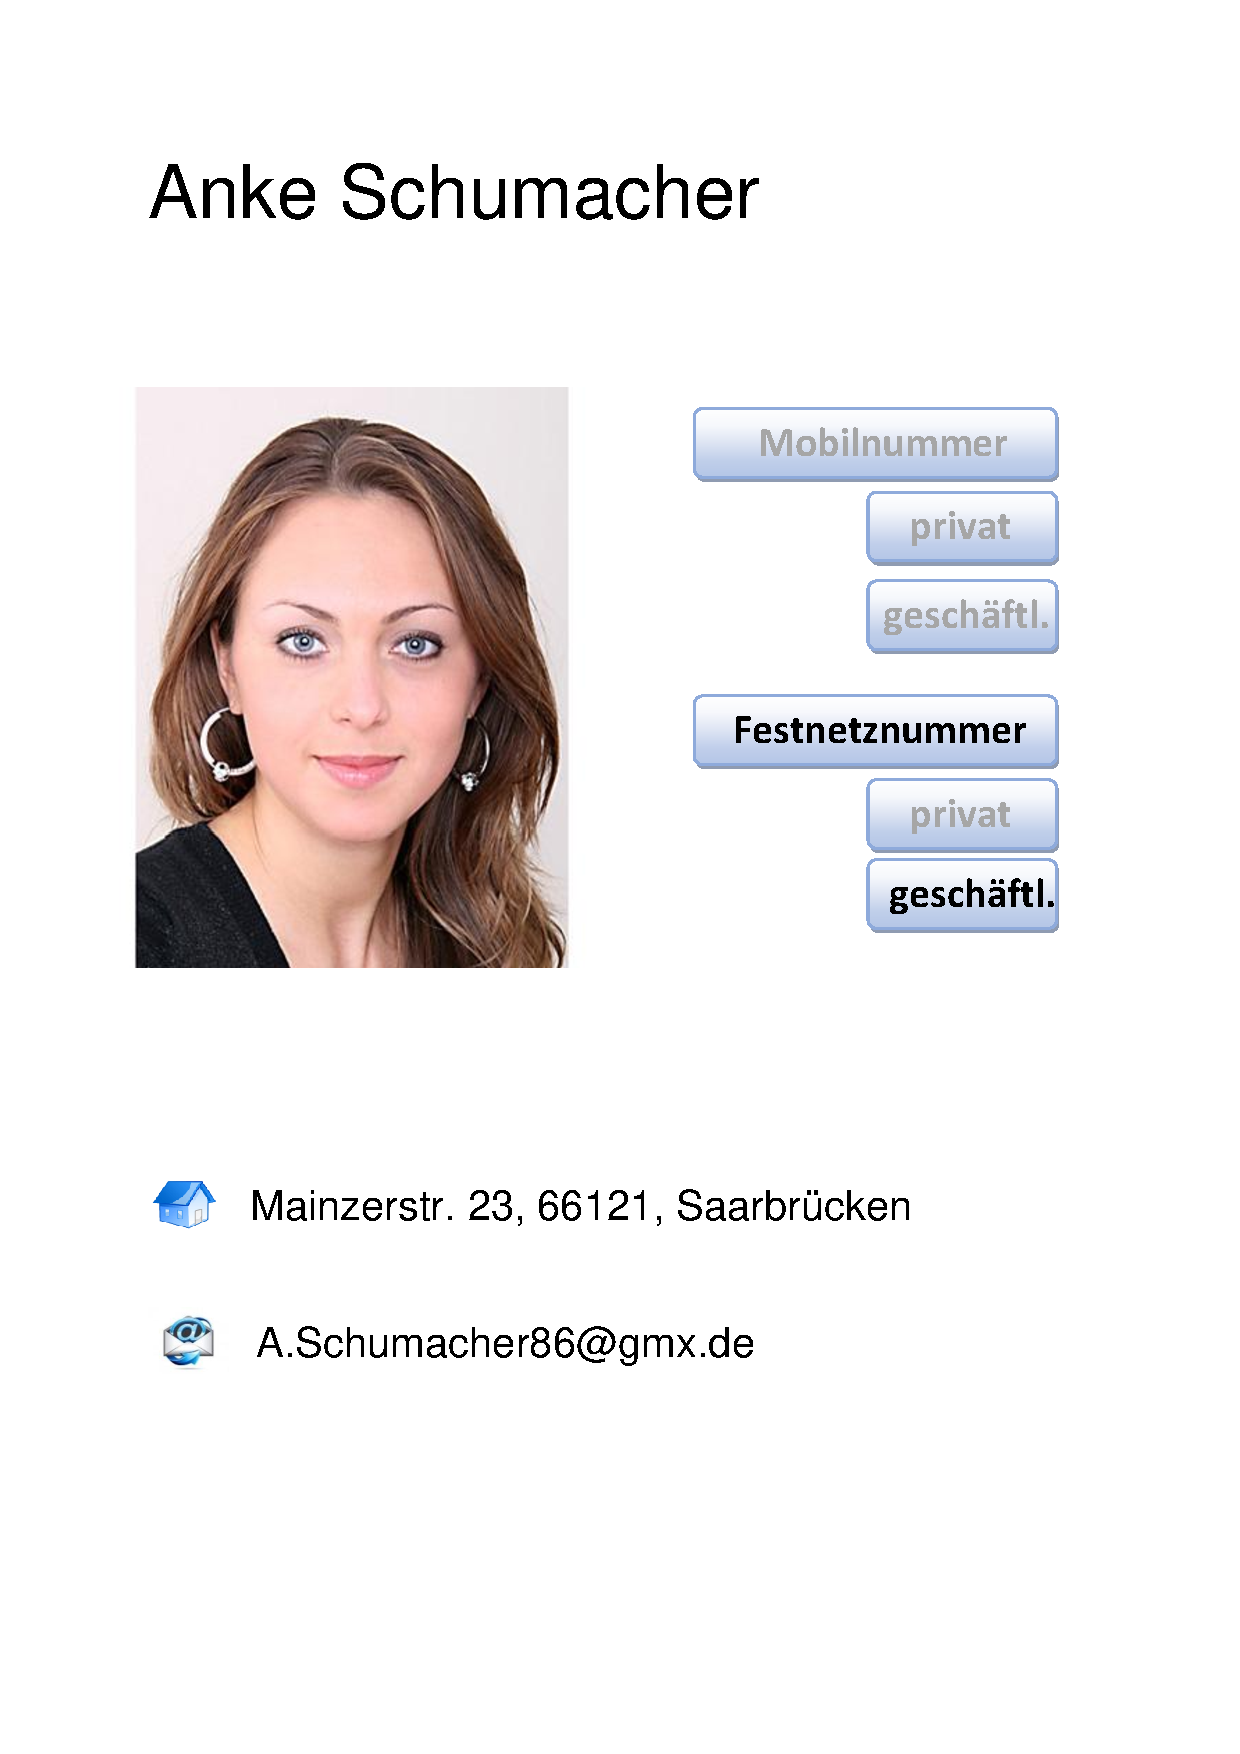
\includegraphics[width=12cm]{Anke.pdf}
\caption{Personenprofil: Anke}
\label{anke}
\end{center}
\end{figure}
Die Versuchspersonen werden am Anfang darauf hingewiesen, dass sie die Slots einzeln übergeben sollen. Nachdem der User spezifiziert hat, welchen Anrufer er anrufen möchte, fragt das System selbst die erforderlichen Slots ab. Diese Nachfrage wird in den unterschiedlichen Dialogstrategien erfragt. Pro Anruf gibt es insgesamt zwei zu füllende Slots, die mit der selben Disambiguierungsstrategie abgefragt werden. Beim nächsten Anruf muss die Versuchsperson andere Slots füllen und die Nachfrage erfolgt mit der nächsten Strategie. 
Die zu füllenden Slots sind in Tabelle \ref{slots} aufgelistet. Welche Slots pro Person abgefragt werden, zeigt Tabelle \ref{slotsPerson}.

\begin{longtable}{p{6cm}p{8cm}}
	\label{slots}\\
	\caption[Slotabfragen]{Beispiel Slotabfragen}\\
	\hline
	\textbf{Slot} &	\textbf{erfragte Werte}\\
	\hline
	\endfirsthead
	\hline
	\textbf{Slot} &	\textbf{erfragte Werte}\\
	\hline
	\endhead
Nummernytyp & privat oder geschäftlich?\\
Telephontyp & Mobilnummer oder Festnetznummer\\
Nachname & Meier oder Müller\\
Stadt & München oder Ingolstadt\\


\hline
\end{longtable}


\begin{longtable}{p{3,2cm}p{3,2cm}p{3,2cm}p{3,2cm}}
	\label{slotsPerson}\\
	\caption[Slotabfrage pro Person]{Slotabfrage pro Person}\\
	\hline
	\textbf{Anke}&\textbf{Peter}&\textbf{Fritz} &\textbf{Kim}\\
	\hline
	\endfirsthead
	\hline
	\textbf{Anke}&\textbf{Peter}&\textbf{Fritz} &\textbf{Kim}\\
	\hline
	\endhead
Nummerntyp & & Nummerntyp & Nummerntyp\\
Telephontyp & Telephontyp & & Telephontyp \\
& Nachname & & \\
& & Stadt & \\

\hline
\end{longtable}


\subsection{Versuchsaufbau}
Um eine möglichst realistische Fahrsimulation mit hoher kognitiver Belastung darzustellen, werden die Versuchspersonen ein Rennspiel mit einem Racing Wheel und den dazugehörigen Pedalen spielen. Bei dem Rennspiel handelt es sich um \texttt{Need for Speed: Shift}\footnote{\label{foot:nfs}\url{http://www.needforspeed.com/de_DE/shift}}, welches im Einzelrennen - Modus mit jeweils drei Gegnern gefahren wird. Die Versuchspersonen bekommen neben der Systeminteraktion die Aufgabe, eine möglichst hohe Platzierung zu erreichen. Dies soll die Konzentration und damit die kognitive Belastung während dem Rennspiel steigern. Zu Beginn des Versuchs fahren die Probanden zunächst eine Testrunde. Mit dem Ergebnis dieser Runde kann man einschätzen wie gut die jeweiligen Personen im Rennspiel sind und weiter die Schwierigkeit des Spiels, und damit die Rennfähigkeiten der Gegner einstellen. In den nächsten drei Runden werden die Versuchspersonen parallel zum Rennspiel das Testszenario durchgehen und dabei drei Personen anrufen. 

 Der Anruf gilt nur dann als erfolgreich, wenn alle Slots korrekt gefüllt werden. 
In der letzten Runde findet nur eine Systeminteraktion statt, ohne paralleles Rennspiel und die dadurch verursachte kognitive Belastung. 
Tabelle \ref{ablauf} zeigt einen Überblick des Versuchsaufbaus.

\begin{longtable}{p{2,4cm}p{2,4cm}p{2,4cm}p{2,4cm}p{2,4cm} }
	\label{ablauf}\\
	\caption[Übersicht Versuchsablauf]{Übersicht Versuchsablauf}\\
	\hline
	\textbf{1. Runde}&\textbf{2. Runde}&\textbf{3. Runde} &\textbf{4. Runde} & \textbf{5. Runde}\\
	\hline
	\endfirsthead
	\hline
	\textbf{1. Runde}&\textbf{2. Runde}&\textbf{3. Runde} &\textbf{4. Runde} \textbf{5. Runde}\\
	\hline
	\endhead
Rennspiel & Rennspiel & Rennspiel & Rennspiel &\\
 & Anruf Anke & Anruf Peter & Anruf Fritz & Anruf Kim \\
\hline
\end{longtable}
Während des Versuchs wird die Versuchsperson, das Rennspiel und die Dialoginteraktion aufgezeichnet. Dadurch wird sicher gestellt, dass man alle Reaktion einfangen und die Daten besser auswerten kann. 

\subsection{Versuchsdesign}
Die Versuchspersonen fahren in den Runden 2-4 jeweils eine Strecke mit unterschiedlicher Disambiguierungsstrategie. Insgesamt werden diese auf drei unterschiedliche Strecken verteilt. Man hat sich für drei unterschiedliche Strecken entschieden, da man einen Lerneffekt bei einer gleichbleibenden Strecke ausschließen wollte. Parallel  werden die Zeiten gemessen, die eine Versuchsperson für die Absolvierung einer Strecke bei der Interaktion mit einer bestimmten Disambiguierungsstrategie benötigt (siehe Unterkapitel \ref{messwerte}). Da man diese Zeiten miteinander vergleichen möchte, müssen die Disambiguierungsstrategien geschickt auf die Strecken verteilt werden, da die Strecke unterschiedlich lang sind und daher keine aussagekräftigen Vergleiche untereinander bieten. Um diesen Konflikt zu lösen, werden die Versuchspersonen in drei Gruppen aufgeteilt, sodass jede Gruppe jede Strecke mit einer unterschiedlichen Disambiguierungsstrategie fährt. Schließlich kann man so für jede Strecke die Zeiten für unterschiedliche Strategien sammeln und vergleichen, mit welcher Strategie eine bestimmte Strecke am schnellsten gefahren wurde (siehe Kapitel \ref{messwerte} Auswertung). \\
In der letzten Runde soll nur das Testszenario ohne Rennspiel durchgeführt werden. Hierfür gibt es Gruppe 4, welche aus allen Versuchsteilnehmern besteht. Diese wird jedoch nochmal in drei Zwischengruppen aufgeteilt, sodass ein drittel der Versuchspersonen in der vierten Runde das Testszenario in Strategie 1, ein drittel in Strategie 2 und das letzte drittel in Strategie 3 durchführen. Ein Überblick der Strecken- und Strategieverteilung pro Gruppe ist in Tabelle \ref{ablauf} aufgelistet. 

\subsection{Control Panel}
Um ein laufendes System zu simulieren wurde ein Control Panel entwickelt, welches verschiedene Sprachausgaben per Mausklick triggert. Damit kann der Versuchsleiter, der Wizard, die passenden Sprachausgaben auf entsprechende Benutzereingaben auslösen. Neben Ausgaben für die einzelnen Disambiguierungsstrategien sind weitere Sprachausgaben abgedeckt, welche oberflächlich zu jeder Eingabe des Benutzers eine Antwort bereit stellen und somit einen ungehinderten Ablauf des Dialogs gewährleisten. Zusätzlich dazu ist ein Stoppbutton enthalten, mit welchem per Klick alle aktiven Sprachausgaben abgebrochen werden können. 
Das Control Panel wurde mit JavaFx\footnote{\label{foot:javafx}\url{http://docs.oracle.com/javase/8/javase-clienttechnologies.htm}} entwickelt. Mit Hilfe des Programms JavaFX Scene Builder\footnote{\label{foot:fxsb}\url{http://www.oracle.com/technetwork/java/javase/downloads/javafxscenebuilder-info-2157684.html}} wurde zunächst das Design entwickelt und in einer .fxml Datei gespeichert. Diese wurde anschließend in Eclipse unter Installation des Plugins E(fx)clipse geladen und die Funktionen für die Sprachausgaben und des Stopp-Buttons implementiert. Die Sprachausgaben wurden online auf der Webseite \url{http://www.fromtexttospeech.com/} als .mp3 Datei generiert und anschließend zu .wav Dateien konvertiert. 
Abbildung \ref{cp1} zeigt das Control Panel. Für jede anzurufende Person gibt es ein extra Tab mit speziellen Sprachausgaben. Die gemeinsamen Sprachausgaben wie \texttt{Cancel} und der Stoppbutton sind in jedem Personentab extra enthalten, damit eine schnelle Reaktion des Versuchsleiters möglich ist. Das Commonstab enthält die Begrüßungsausgabe. Zur Orientierung ist nach jedem speziellen Button die ausgelöste Sprachausgabe zu sehen. 
\begin{figure}[htbp]
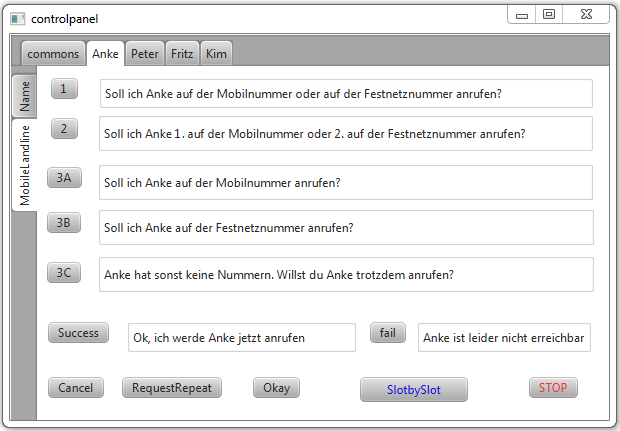
\includegraphics{controlpanel.png}
\caption{Controlpanel}
\label{cp1}
\end{figure}

\begin{longtable}{p{3cm}p{3cm}p{3cm}p{3cm} }
	\label{ablauf}\\
	\caption[Strecken- und Strategieverteilung]{Strecken- und Strategieverteilung}\\
	\hline
	\textbf{Aufteilung}&\textbf{Strategie 1}&\textbf{Strategie 2} &\textbf{Strategie 3}\\
	\hline
	\endfirsthead
	\hline
	\textbf{Aufteilung}&\textbf{Strategie 1}&\textbf{Strategie 2} &\textbf{Strategie 3}\\
	\hline
	\endhead
1. Gruppe & Strecke A & Strecke B & Strecke C \\
2. Gruppe & Strecke B & Strecke C & Strecke A \\
3. Gruppe  & Strecke C & Strecke A & Strecke B \\
4. Gruppe   & keine Strecke & keine Strecke & keine Strecke\\ 
\hline
\end{longtable}

Jede Gruppe fährt die Strecken in der gleichen Reihenfolge (erst Strecke A dann Strecke B und schließlich Strecke C). Dadurch soll gewährleistet sein, dass die Streckenzeiten durch keinen Lerneffekt bei einer unterschiedlicher Reihenfolge beeinflusst werden. Wenn Strecke A mal zu Beginn und mal zum Schluß gefahren wird, so könnten die Zeiten für die Runde am Schluß besser ausfallen, da die Versuchsperson durch die vorherigen Runden mehr an Spielererfahrung gewonnen hat und bessere Zeiten fährt. Die anzurufenden Personen sind auf bestimmte Strecken festgelegt und in Tabelle \ref{anrufstrecke} gelistet. 

\begin{longtable}{p{6cm}p{6cm}}
	\label{anrufstrecke}\\
	\caption[Anruf per Strecke]{Anruf per Strecke}\\
	\hline
	\textbf{Strecke} &	\textbf{Anruf}\\
	\hline
	\endfirsthead
	\hline
	\textbf{Strecke} &	\textbf{Anruf}\\
	\hline
	\endhead
Strecke A & Anke\\
Strecke B & Peter\\
Strecke C & Fritz\\
keine Strecke & Kim\\


\hline
\end{longtable}

\subsection{Versuchspersonen}
Es wurden 12 Versuchspersonen getestet. Davon waren sieben in der Altersgruppe 18-29, zwei in der Altersgruppe 30-41 und drei in der Altergruppe 42-53. Alle Veruschpersonen waren deutsche Muttersprachler. Unter diesen Personen haben zwei Erfahrung mit Dialogsystemen, zwei spielen öfter Rennspiele und fünf fiel die Einführungsrunde einfach. Zu Beginn wurden die Versuchspersonen in eine Gruppe aufgeteilt, durch die bestimmt wird, welche Strategie auf welcher Strecke gefahren wird (siehe Tabelle \ref{ablauf}.
Der Versuchsablauf für die Versuchsperson sah folgendermaßen aus:
\begin{enumerate}
\item Testrunde fahren
\item Fragebogen über Person ausfüllen (siehe \ref{fbperson1})
\item Strecke A fahren + Anke anrufen
\item Fragebogen über kognitive Belasung und letzten Dialog ausfüllen (siehe \ref{fbnasatlx1} und \ref{fbstrategien1} )
\item Strecke B fahren + Peter anrufen
\item Fragebogen über kognitive Belasung und letzten Dialog ausfüllen
\item Strecke C fahren + Fritz anrufen
\item Fragebogen über kognitive Belasung und letzten Dialog ausfüllen 
\item Kim anrufen
\item Fragebogen über kognitive Belasung und letzten Dialog ausfüllen 
\end{enumerate}

Den Versuchpersonen wurde mitgeteilt, dass sie mit einem echten System interagieren und darum gebeten, während des Dialogs deutlich in ein Tischmikrofon zu sprechen. Die Personenprofile konnten sie während des Dialoges über einen Laptop ansehen.

\subsection{Auswertung}
\label{auswertung1}
Um herauszufinden, welche Disambiguierungsstrategie am effizientesten ist, werden verschiedene Auswertungen vorgenommen. 
Zunächst werden die Zeiten gemessen, die die Versuchsperson zum einen für das absolvieren der Strecke und zum anderen für das erfolgreiche abschließen des Testszenarios benötigt (Unterkapitel \ref{messwerte}).
Außerdem werden die Fragebogen ausgewertet, die von den Versuchsperson nach jeder Runde ausgefüllt werden. Diese beziehen sich auf die subjektiv wahrgenommene kognitive Belastung und auf Merkmale der Disambiguierungsstrategien (Unterkapitel \ref{fragebogen}). Desweiteren wird die Task Completion ausgewertet um zu erforschen, wie erfolgreich ein Dialog geführt wurde. Schließlich wird überprüft, wie die Versuchspersonen auf Rückfragen geantwortet haben und ob es dabei einen Unterschied zwischen hoch und niedrig belastenden Personen gibt. 
\subsubsection{gemessene Zeiten}
\label{messwerte}
\paragraph{Rennzeiten} 
~\\
%\textbf{Rennzeiten}\\
Um zu analysieren, ob das Rennverhalten durch eine Disambiguierungsstrategie negativ beeinflusst wird, werden die Rennzeiten pro Runde gemessen. Für jede Strecke wird dann die durchschnittliche Zeit gebildet, die die Versuchspersonen mit paralleler Systeminteraktion in einer bestimmten Strategie benötigten. Das Ergebnis ist in Tabelle \ref{RZ3SV1} aufgelistet.

\begin{longtable}{p{3cm}p{3cm}p{3cm}p{3cm} }
	\label{RZ3SV1}\\
	\caption[Durchschnittszeiten Strategie pro Strecke]{Durchschnittszeiten Strategie pro Strecke}\\
	\hline
	\textbf{Rennzeiten}&\textbf{Strategie 1}&\textbf{Strategie 2} &\textbf{Strategie 3}\\
	\hline
	\endfirsthead
	\hline
	\textbf{Rennzeiten}&\textbf{Strategie 1}&\textbf{Strategie 2} &\textbf{Strategie 3}\\
	\hline
	\endhead
Strecke A & 71,5 sek & 93 sek & 74,5 sek \\
Strecke B & 68,75 sek & 75,75 sek & 91,5 sek \\
Strecke C & 74,5 sek & 58,38 sek & 61,75 sek \\
\hline
\end{longtable}

Diesen Ergebnissen zufolge, gibt es keine Strategie, mit der eine Strecke besser oder schlechter gefahren wurde als mit anderen Strategien. 
Dies könnte jedoch daran liegen, dass einzelnen Werte durch schlechtere bzw. bessere Spieler in den Gruppen verfälscht wurden.
Befindet sich zum Beispiel ein sehr schlechter Spieler in Gruppe 1 und ein sehr guter Spieler in Gruppe 2, so könnte die Durchschnittszeit für Strategie 1 auf Strecke A, durch die lange Zeit des schlechten Spielers, verschlechtert werden. Im Gegensatz dazu könnte die Durchschnittszeit für Strategie 3 auf Strecke A durch die guten Resultate des guten Spielers aus Gruppe 3 verbessert werden. Um dieses Problem zu lösen, wird pro Strategie der Durchschnitt aller mit dieser Strategie gefahrenen Rennzeiten berechnet. Zeiten von extrem guten bzw. schlechten Spielern sollten die Durchschnittszeiten ganzer Strategien dann nicht mehr beeinflussen. Die daraus resultierenden Werte geben dann eine Aussage darüber, mit welcher Strategie die Rennen am besten bzw. am schlechtesten gefahren wurden. 
Die endgültige Rennzeitberechnung für die Analyse der effizientesten Disambiguierungsstrategie ist in Tabelle \ref{RennZeitenDis1} dargestellt.

\begin{longtable}{p{3cm}p{3cm}p{3cm}p{3cm} }
	\label{RennZeitenDis1}\\
	\caption[Durschnittszeiten pro Strategie]{Durschnittszeiten pro Strategie}\\
	\hline
	\textbf{Rennzeiten}&\textbf{Strategie 1}&\textbf{Strategie 2} &\textbf{Strategie 3}\\
	\hline
	\endfirsthead
	\hline
	\textbf{Rennzeiten}&\textbf{Strategie 1}&\textbf{Strategie 2} &\textbf{Strategie 3}\\
	\hline
	\endhead
Durschnitt & 71,58 sek & 75,71 sek & 75,92 sek\\
\hline
\end{longtable}
Die Unterschiede der Rennzeiten der einzelnen Strategien sind jedoch statistisch nicht relevant (p = 0,79). Daher kann hier nicht der Rückschluss gezogen werden, dass Strategie 1 die Versuchspersonen am wenigstens ablenkt. Desweiteren steht die Frage offen, ob die Rennzeiten überhaupt Ausschluss darüber geben können, welche Strategie sich am besten während der Autofahrt eignet. Dies könnte in zukünftigen Arbeiten durch einen umfangreicheren Versuch überprüft werden. Möglicherweise könnten besser Ergebnisse erzielt werden, wenn die Rennstrecken kürzer gewählt werden.  


\begin{comment}
\begin{longtable}{p{3cm}p{3cm}p{3cm}p{3cm} }
	\label{durchschnittsvorl}\\
	\caption[Durschnittszeiten Strategie pro Strecke]{Durschnittszeiten Strategie pro Strecke}\\
	\hline
	\textbf{Rennzeiten}&\textbf{Strategie 1}&\textbf{Strategie 2} &\textbf{Strategie 3}\\
	\hline
	\endfirsthead
	\hline
	\textbf{Rennzeiten}&\textbf{Strategie 1}&\textbf{Strategie 2} &\textbf{Strategie 3}\\
	\hline
	\endhead
Strecke A & sek \O & sek \O & sek \O \\
Strecke B & sek \O & sek \O & sek \O\\
Strecke C  & sek \O & sek \O & sek \O\\

\hline
\end{longtable}


Tabelle \ref{durchschnittsvorl} ist nur eine Übergangstabelle, da  einzelnen Werte durch schlechte Spieler in den Gruppen verfälscht werden können. Befindet sich zum Beispiel ein sehr schlechter Spieler in Gruppe 1 und ein sehr guter Spieler in Gruppe 2, so könnte die Durschnittszeit für Strategie 1 auf Strecke A, durch die lange Zeit des schlechten Spielers, verschlechtert werden. Im Gegensatz dazu könnte die Durschnitsszeit für Strategie 3 auf Strecke A durch die guten Resultate von dem guten Spieler aus Gruppe 3 verbessert werden. Um dieses Problem zu lösen, nimmt man die Durchschnittszeiten aus Tabelle \ref{durchschnittsvorl} noch mal zum Durschnitt und erhält so eine Durschnittszeit pro Strategie. Die daraus resultierenden drei Werte sagen dann aus, mit welcher Strategie die Rennen am besten gefahren wurden. Zeiten von extrem guten bzw. schlechten Spielern sollten die Durschnittszeiten einzelner Strecken dann nicht mehr beeinflussen.  
Die endgültige Zeitberechnung für die Analyse der effizientesten Disambiguierungsstrategie ist in Tabelle \ref{ZeitenDis} dargestellt.
\end{comment}


\paragraph{Dialogzeiten}
~\\
Neben den Zeiten für das Rennspiel werden auch die Dialogzeiten berechnet. Anhand dieser Zeiten kann man sehen, mit welcher Strategie der kürzeste Dialog möglich ist. Desweiteren kann man die Dialogzeiten vergleichen, die einmal in der gleichen Strategie mit Rennspiel und einmal ohne Rennspiel erzielt wurden. Das könnte interessant sein, um die Unterschiede im Dialogverhalten zwischen einer kognitiv hoch belastenden Versuchsperson und einer weniger belastenden Person zu untersuchen. Eine längere Dialogzeit in einer gleichen Strategie ist möglicherweise auf eine längere Reaktionszeit zurückzuführen, weshalb bessere Zeiten in der vierten Runde, also ohne Rennspiel und damit ohne hohe kognitive Belastung, erwartet werden. Es werden alle Dialogzeiten aus den Runden mit Rennspiel gemessen und einmal für jede Strecke der Durchschnitt pro Strategie und einmal der gesamte Durchschnitt pro Strategie gebildet. Diese Werte kann man dann gegen die Durchschnittszeiten aus der Runde ohne Rennstrecke vergleichen. Es werden allerdings nur die Dialogzeiten bewertet, bei denen der Dialog korrekt durchgeführt wurde, da sonst die Durchschnittszeiten verfälscht werden können.  Tabelle \ref{Durchschnittsdialogzeiten1} zeigt die Ergebnisse.

\begin{longtable}{p{3cm}p{3cm}p{3cm}p{3cm} }
	\label{Durchschnittsdialogzeiten1}\\
	\caption[Durchschnittsdialogzeiten]{Durchschnittsdialogzeiten}\\
	\hline
	\textbf{Dialogzeiten}&\textbf{Strategie 1}&\textbf{Strategie 2} &\textbf{Strategie 3}\\
	\hline
	\endfirsthead
	\hline
	\textbf{Rennzeiten}&\textbf{Strategie 1}&\textbf{Strategie 2} &\textbf{Strategie 3}\\
	\hline
	\endhead
Strecke A & 15,34 sek & 20,38 sek & 20,28 sek \\
Strecke B & 14,31 sek & 20,05 sek & 22,07 sek \\
Strecke C  & 15,97 sek & 21,01 sek & 20,35 sek \\
\hline
\hline
Strecke A - C & 15,19 sek & 20,52 sek & 20,81 sek \\
\hline
ohne Strecke &  14,9 sek & 18,8 sek & 17,59 sek \\
\hline
\end{longtable}

Die Unterschiede aus Strategie 1 sind statistisch signifikant gegenüber den Unterschieden aus Strategie 2 und 3. Die Unterschiede aus Strategie 2 und 3 sind zueinander jedoch nicht signifikant. Das Ergebnis zeigt, dass die Strategie 1 den kürzesten Dialog sowohl mit Rennspiel, als auch ohne Rennspiel ermöglicht. Die letzten beiden Zeilen der Tabelle zeigen, dass die Versuchspersonen einen deutlich kürzeren Dialog in jeder Strategie ohne Rennspiel ablegen. Die Ergebnisse aus dem Unterkapitel \ref{Dialogverhalten1} lassen ausschließen, dass die Unterschiede aufgrund eines unterschiedlichen Dialogverhaltens zu erklären sind. Dies lässt vermuten, dass die Reaktionszeiten bei geringer Belastung kleiner sind als bei hoher Belastung und die zeitlichen Unterschiede dadurch zu Stande kommen. 
\subsubsection{Fragebogen}
\label{fragebogen}
Neben den Zeiten wird nach jeder Runde ein Fragebogen ausgefüllt. Dieser besteht im ersten Teil aus einem Ausschnitt des NASA-TLX Testes zur subjektiven Einschätzung der empfundenen kognitiven Belastung. Im zweiten Teil werden Fragen über die zuletzt getestete Strategie gestellt und es wird die Möglichkeit gegeben positives oder negatives Feedback über den Dialog der letzten Runde zu geben. Zu Beginn des Versuchs wird ein allgemeiner Fragebogen ausgefüllt, der Informationen zur Versuchsperson liefert. 
\paragraph{Nasa-TLX}
~\\
Abbildung \ref{fbnasatlx} zeigt den Nasa-TLX Teil des ersten Fragebogens. 
\begin{figure}[htbp]
\begin{center}
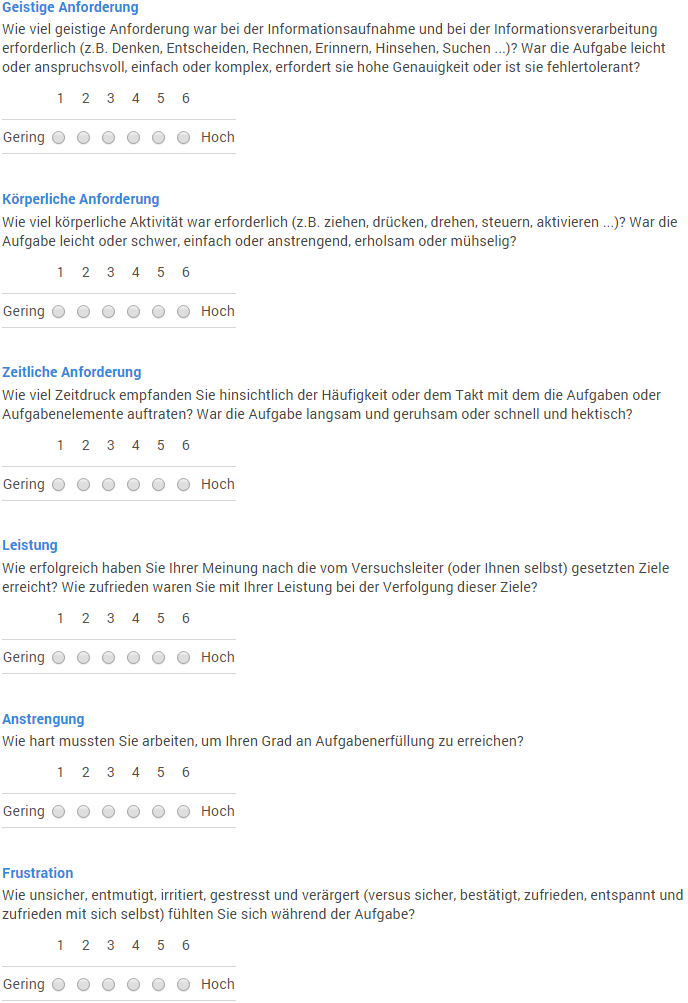
\includegraphics[width=12cm]{nasa.png}
\caption{Fragebogen: Nasa-TLX}
\label{fbnasatlx1}
\end{center}
\end{figure}
Die Ergebnisse dieses Testes werden zum Einen dafür genutzt um zu erforschen, bei welcher Strategie die Versuchspersonen eine höhere kognitive Belastung empfunden haben. Zum anderen kann man sehen, wie die Versuchspersonen ihre kognitive Belastung während einer Runde mit Rennspiel im Vergleich zur Runde ohne Rennspiel einschätzen. 
Die Nachfolgende Tabelle zeigt die Ergebnisse jeder Frage pro Strategie. Dabei werden jeweils die durchschnittlichen Antworten für alle Runden, der Runden mit Rennspiel und nur der Runde ohne Rennspiel aufgelistet. 
\newline
\begin{longtable}{|p{4cm}|p{2cm}|p{2cm}|p{2cm}|p{2cm}|}
	\hline
		\textbf{Antwortenintervall}&\textbf{Strategien}&\multicolumn{3}{c|}{\textbf{Ergebnisse bestimmter Runden}}\\
	&&\textbf{1-4}&\textbf{1-3} &\textbf{4}\\
	\hline
	\endfirsthead
	\hline
	\textbf{Antwortenintervall}&\textbf{Strategien}&\textbf{Runden 1-4}&\textbf{Runden 1-3} &\textbf{Runde 4}\\
	\hline
	\endhead
		\multicolumn{5}{l}{\textbf{Geistige Anforderung}}\\
		\hline
\multirow{3}{4cm}{1: gering \newline 6: hoch} & Strategie 1 &  1,88 & 2,08 & 1,25 \\
 & Strategie 2 & 2,06 & 2,42 & 1\\
 & Strategie 3 & 2,63 & 2,83 & 2 \\
\hline
		\multicolumn{5}{l}{\textbf{Körperliche Anforderung}}\\
		\hline
\multirow{3}{4cm}{1: gering \newline 6: hoch} & Strategie 1 & 2 & 2,17 & 1,5 \\
 & Strategie 2 & 1,44 & 2,25 & 1 \\
 & Strategie 3 & 2 & 2,25 & 1,25 \\
\hline
		\multicolumn{5}{l}{\textbf{Zeitliche Anforderung}}\\
		\hline
\multirow{3}{4cm}{1: gering \newline 6: hoch} & Strategie 1 & 1,87 & 2,09 & 1,25 \\
 & Strategie 2 & 1,75 & 2 & 1 \\
 & Strategie 3 & 2,31 & 2,67 & 1,25 \\
\hline
		\multicolumn{5}{l}{\textbf{Leistung}}\\
		\hline
\multirow{3}{4cm}{1: gering \newline 6: hoch} & Strategie 1 & 4,25 & 4,5 & 3,5 \\
 & Strategie 2 & 4,75 & 4,33 & 6 \\
 & Strategie 3 & 4,25 & 4 & 5 \\
\hline
		\multicolumn{5}{l}{\textbf{Anstrengung}}\\
		\hline
\multirow{3}{4cm}{1: gering \newline 6: hoch} & Strategie 1 & 2 & 2,25 & 1,25 \\
 & Strategie 2 & 2,13 & 2,55 & 1 \\
 & Strategie 3 & 2,63 & 2,92 & 1,75\\
\hline
		\multicolumn{5}{l}{\textbf{Frustration}}\\
		\hline
\multirow{3}{4cm}{1: gering \newline 6: hoch} & Strategie 1 & 1,69 & 1,83 & 1,25 \\
 & Strategie 2 & 1,81 & 2,08 & 1 \\
 & Strategie 3 & 2 & 2,25 & 1,25 \\
\hline
\end{longtable}

Die Unterschiede der Antworten einzelner Strategien sind nicht signifikant, sodass nicht eindeutig gesagt werden kann, welche Strategie die Versuchsperson am meisten bzw. am wenigsten belastet. Betrachtet man jedoch die Ergebnisse aller Fragen fällt auf, dass die Ergebnisse für die geistige Anforderung, die Anstrengung und die Frustration zeigen, dass die erste Strategie am unbelastendsten und die dritte Strategie am belastendsten gewertet wurde. Dies deckt sich auch mit den Ergebnissen aus dem Strategien Fragebogen, in dem die erste Strategie als Favorit und die dritte Strategie als unbeliebteste Strategie gewertet wurde. Vergleicht man die Werte für Runde 1-3 mit den Werten von Runde 4 fällt auf, dass die Dialoge parallel zum Rennspiel mit Ausnahme der Frage nach der Leistung durchweg als belastender gewertet wurden als die Dialoge ohne Rennspiel. Dies zeigt, dass die Versuchspersonen einen Unterschied in der kognitiven Belastung gespürt haben.   
\paragraph{Strategien}
~\\
Der zweite Teil des Fragebogens ist in Abbildung \ref{fbdialog} zu sehen. 
\newline
\begin{figure}[htbp]
\begin{center}
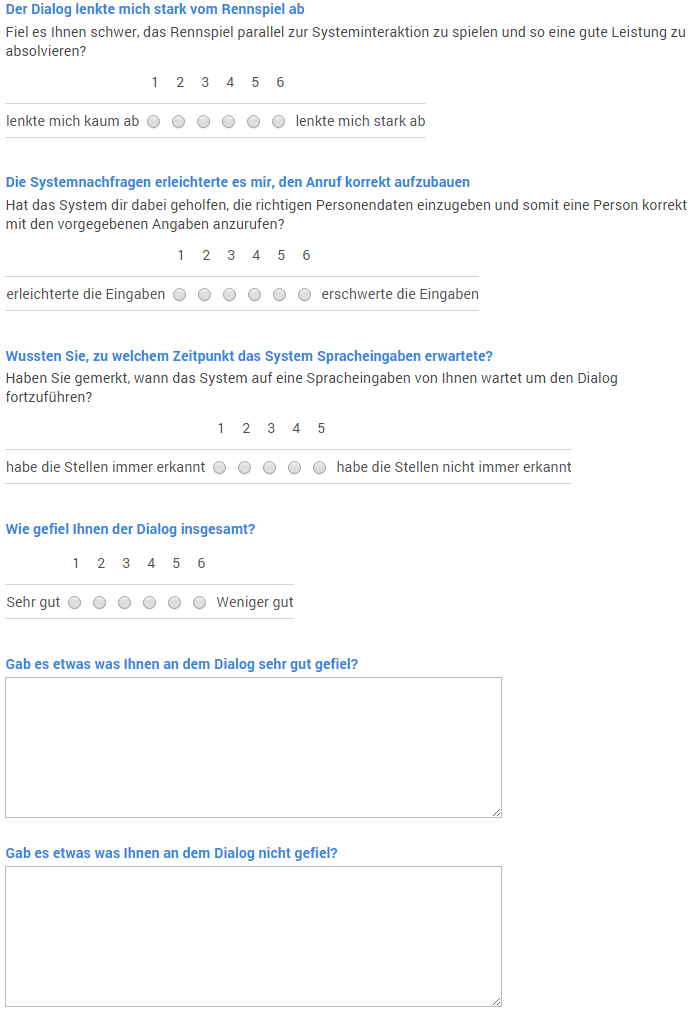
\includegraphics[width=12cm]{fbdialog.png}
\caption{Fragebogen: Dialogverhalten}
\label{fbstrategien1}
\end{center}
\end{figure}

In diesem Teil geht es darum, die einzelnen Strategie anhand verschiedener Kategorien zu bewerten.
Die Nachfolgende Tabelle zeigt die Ergebnisse jeder Frage pro Strategie. Dabei werden jeweils die durchschnittlichen Antworten für alle Runden, der Runden mit Rennspiel und nur der Runde ohne Rennspiel aufgelistet. 
\newline

\begin{longtable}{|p{4cm}|p{2cm}|p{2cm}|p{2cm}|p{2cm}|}
	\hline
		\textbf{Antwortenintervall}&\textbf{Strategien}&\multicolumn{3}{c|}{\textbf{Ergebnisse bestimmter Runden}}\\
	&&\textbf{1-4}&\textbf{1-3} &\textbf{4}\\
	\hline
	\endfirsthead
	\hline
	\textbf{Antwortenintervall}&\textbf{Strategien}&\textbf{Runden 1-4}&\textbf{Runden 1-3} &\textbf{Runde 4}\\
	\hline
	\endhead
		\multicolumn{5}{l}{\textbf{Der Dialog lenkte mich vom Rennspiel ab}}\\
		\hline
\multirow{3}{4cm}{1: kaum \newline 6: stark} & Strategie 1 & \multirow{3}{2,5cm}{in Runde 4 nicht beantwortet} & 2,25  & \multirow{3}{2,5cm}{nicht beantwortet} \\
 & Strategie 2 & & 2,58 & \\
 & Strategie 3 & & 2,58 & \\
\hline
		\multicolumn{5}{l}{\textbf{Die Nachfragen erleichterten es mir, den Anruf korrekt aufzubauen}}\\
		\hline
\multirow{3}{4cm}{1: erleichterte es\newline  6: erschwerte es} & Strategie 1 & 1,63 & 1,83 & 1,25 \\
 & Strategie 2 & 1,69 & 1,92 & 1 \\
 & Strategie 3 & 2,13 & 2,25 & 1,75 \\
\hline
		\multicolumn{5}{l}{\textbf{Wussten Sie, wann das System Spracheingaben erwartete?}}\\
		\hline
\multirow{3}{4cm}{1: immer \newline  6: nicht immer} & Strategie 1 & 1,19 & 1,17 & 1,25 \\
 & Strategie 2 & 1,38 & 1,33 & 1,5 \\
 & Strategie 3 & 1,5 & 1,67 & 1 \\
\hline
		\multicolumn{5}{l}{\textbf{Wie gefiel Ihnen der Dialog insgesamt?}}\\
		\hline
\multirow{3}{4cm}{1: sehr gut \newline  6: weniger gut} & Strategie 1 & 1,94 & 2,08 & 1,5 \\
 & Strategie 2 & 2,50 & 2,67 & 2 \\
 & Strategie 3 & 2,57 & 2,75 & 2 \\
\hline
		\multicolumn{5}{l}{\textbf{Fiel es Ihnen einfacher, den Dialog ohne Rennspiel zu führen?}}\\
		\hline
\multirow{3}{4cm}{1: viel einfacher \newline  6: nicht einfacher} & Strategie 1 & \multirow{3}{2,5cm}{in Runden 1-3 nicht beantwortet} & \multirow{3}{2,5cm}{nicht beantwortet} & 2 \\
 & Strategie 2 & & & 3,75 \\
 & Strategie 3 & & & 2,25\\
\hline
		\multicolumn{5}{l}{\textbf{Welcher Anruf gefiel Ihnen insgesamt am besten?}}\\
		\hline
\multirow{3}{4cm}{Anruf bzw. Strategie auswählbar} & Strategie 1 & 75\% & & \\
 & Strategie 2 & 16,6\% && \\
 & Strategie 3 & 8,3\% && \\
\hline
\end{longtable}

Die ersten vier Antworten dieses Fragebogen zeigen, dass die erste Strategie am positivsten und die dritte Strategie am negativsten gewertet wurden. Dies stimmt mit dem Ergebnis der letzten Frage überein, welche konkret nach der beliebtesten Strategie nachfragt. Die Vorletzte Frage zeigt, dass es dem Durchschnitt der Versuchspersonen einfacher fiel, den Dialog ohne Rennspiel zu führen. Dies bestätigt das Ergebnis aus dem Nasa-TLX Fragebogen, welches besagt, dass ein Unterschied in der kognitiven Belastung zwischen Dialog mit Rennspiel und ohne Rennspiel unter den Versuchspersonen bemerkbar ist.  

\paragraph{Person}
~\\
\label{fbperson1}
In Abbildung \ref{fbperson} sind die Fragen dieses Fragebogens abgebildet.
Die Fragen nach der Rennspiel- und Dialogerfahrung können für die spätere Auswertung der Zeiten interessant sein und eine mögliche Erklärung für stark abweichende Rennspiel- Und Dialogzeiten liefern. 
\begin{figure}[htbp]
\begin{center}
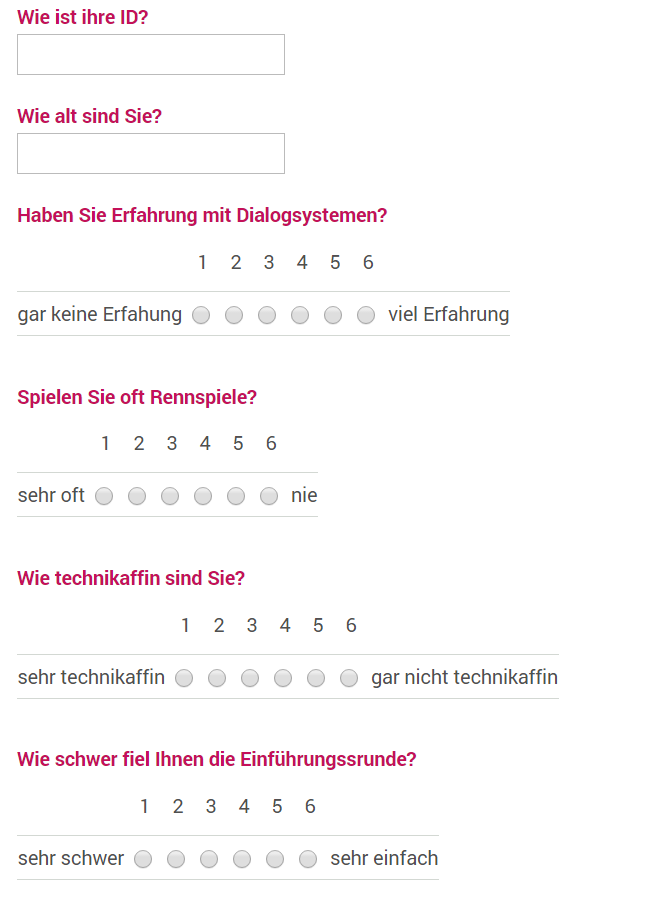
\includegraphics[width=12cm]{fbperson.png}
\caption{Fragebogen: Person}
\label{fbperson}
\end{center}
\end{figure}

\subsubsection{Task Completion}
Für jede Strategie wird die Task Completion ausgewertet, welche besagt, mit welchem Erfolg der Anruf ausgeführt wurde. Sie wird bemessen, in dem man für jeden richtig gefüllten Slot (siehe Tabelle \ref{slotsPerson}) einen Punkt verteilt. Folgenden Punktzahlen sind also für jede Strategie möglich:
\begin{itemize}
\item 0 Punkte, wenn kein Slot richtig gefüllt wird
\item 1 Punkt, wenn ein Slot richtig gefüllt wird
\item 2 Punkte, wenn alle Slots richtig gefüllt wird
\end{itemize}
Zur Auswertung wird pro Strategie eine Durschnittspunktzahl berechnet. 
Diese finden sich in Tabelle \ref{TCV1}.

\begin{longtable}{p{3cm}p{3cm}p{3cm}p{3cm} }
	\label{TCV1}\\
	\caption[Durschnittliche Task Completion (TC)]{Durschnittliche Task Completion (TC)}\\
	\hline
\textbf{Strategien}&\textbf{insgesamt}&\textbf{Runde 1-3} &\textbf{Runde 4}\\
	\hline
	\endfirsthead
	\hline
	\textbf{Strategien}&\textbf{\O TC insgesamt}&\textbf{\O TC Runde 1-3} &\textbf{\O TC Runde 4}\\
	\hline
	\endhead
1. Strategie & 1,75 & 1,92 & 1,5  \\
2. Strategie & 1,94 & 1,92 & 2  \\
3. Strategie & 1,63 & 1,5 & 2  \\
\hline
Insgesamt & & 1,78 & 1,83 \\ 
\hline
\end{longtable}

Im Durchschnitt wurde in der Runde ohne Rennspiel eine höhere Task Completion erreicht. Das besagt, dass die Dialoge der vierten Runde am erfolgreichsten sind. Der Unterschied ist jedoch sehr gering, sodass man für ein eindeutiges Ergebnis mehr Ergebnisse zur Auswertung benötigt. Das Ergebnis zeigt weiter, dass die 2. Strategie insgesamt am erfolgreichsten ist. Die erfolgloseste Strategie ist nach diesem Ergebnis die dritte Strategie. Dies passt zum Ergebnis, dass diese Strategie im 2. Teil des Fragebogen am schlechtesten gewertet wurde. Strategie 1, welche als beliebteste Strategie der Runde 1-3 ausgewählt wurde, liefert für diese Runden die gleiche Task Completion wie Strategie 2. Hier fehlen weitere Ergebnisse um eine konkrete Verbindung zwischen beliebteste Strategie und Strategie mit höchster Task Completion herzustellen. Dabei muss auch der Fall betrachtet werden, dass die Versuchsperson ihre Fehler möglicherweise gar nicht bemerken. Diese Verbindung könnte in einem umfangreichen Experiment in späteren Arbeiten überprüft werden. 
Grundsätzlich kann man aus diesem Ergebnis sehen, dass insgesamt der Anruf am häufigsten korrekt mit Strategie 2 und am seltensten korrekt mit Strategie 3 ausgeführt werden konnte. \newline
Es ist jedoch fraglich, ob die hier entstandenen Fehler auch in einem realen Dialog aufkommen, bei dem die Versuchsperson selbst entscheidet wer auf welcher Nummer angerufen werden soll. Deshalb gibt diese Auswertung nur ein Indiz darauf, welche Strategie möglicherweise am kompliziertesten ist, wenn man vorgeschriebene Werte übermitteln muss. 


\subsubsection{Dialoverhalten}
Für jede Strategie werden die Antworten der Versuchspersonen gesammelt. Dabei wurden folgenden Antworten pro Strategie gesammelt:
\begin{longtable}{p{4cm}p{4cm}p{4cm}}
	\label{Dialogverhalten11}\\
	\caption[Antwortmöglichkeiten1]{Antwortmöglichkeiten1}\\
	\hline
\textbf{Antwort-möglichkeiten}&\textbf{Beispiel \newline Slotabfrage}&\textbf{Beispiel \newline Antwort}\\
	\hline
	\endfirsthead
	\hline
	\textbf{Antwort-möglichkeiten}&\textbf{Beispiel \newline Slotabfrage}&\textbf{Beispiel \newline Antwort}\\
	\hline
	\endhead
Slots  & Willst du Anke privat oder geschäftlich anrufen? & geschäftlich  \\
Position & Willst du Anke 1. privat oder 2. geschäftlich anrufen? & zweitens  \\
ja/nein & Willst du Anke privat anrufen? &  nein\\ 
\hline
\end{longtable}

Die Häufigkeit dieser Antworten pro Stratgie aus Runde 1-3 sind in nachfolgender Tabelle aufgelistet.

\begin{longtable}{p{3cm}p{3cm}p{3cm}p{3cm} }
	\label{Dialogverhalten12}\\
	\caption[Antwortenverteilung pro Strategie]{Antwortenverteilung pro Strategie}\\
	\hline
\textbf{Antwort-möglichkeiten}&\textbf{Strategie 1}&\textbf{Strategie 2} &\textbf{Strategie 3}\\
	\hline
	\endfirsthead
	\hline
	\textbf{Antwortmöglichkeiten}&\textbf{Strategie 1}&\textbf{Strategie 2} &\textbf{Strategie 3}\\
	\hline
	\endhead
Slots & 100\% & 70,8\%\ & 16,7\%  \\
Position & 0\% & 29,2\% & 0\%  \\
ja/nein & 0\% & 0\%  & 83,3 \%  \\
\hline
\end{longtable}

Um zu erforschen, ob sich das Dialogverhalten in Runde 4 ändert, hat man pro Person die Antworten aus der Strategie der 4. Runde mit der entsprechenden Strategie aus den Runden davor verglichen. Die Ergebnisse zeigen, dass die Antwortmöglichkeit bei hoher Belastung die gleiche ist wie bei niedriger Belastung. Dadurch ist kein Unterschied im Dialogverhalten bei unterschiedlicher Belastung erkennbar ist. 

\begin{comment}
\subsection{Hypothesen}
\textbf{beliebt}: kurze Sprachausgabe, kurze Spracheingabe, wenig Aufmerksamkeit \\
\textbf{unbeliebt}: lange Sprachausgaben mit unnötigen Informationen, anstrengendes Zuhören\\
\textbf{hoher CL}: kurze knappe Eingabe (BargeIn, Füllwörter), Confirmations bevorzugt (Related Work) und möglichst viele Pausen (Strat 3)\\
\textbf{kein/niedriger CL}: weniger BargeIn und Füllwörter(Related Work)


\subsection{Simulation und Durchführung}
Versuchspersonen bekommen bestimmte Aufgabe\\
\\
\texttt{Ich habe eine System für das Auto gebaut, mit welchem ihr Telefonieren könnt. Bitte testet mal alle Funktionen des Systems}\\
\\
$\rightarrow$ denken sie haben andere Aufgabe und wissen nicht was eigentlich getestet werden soll.\\
\\
Versuchspersonen sollen also pro Runde einen Kontakt anrufen\\
Dauer einer Runde je nach Können ca. 2-3 Minuten\\
?? Versuchspersonen können/sollen sich vor jeder Runde kurz durchlesen, welche Interaktionen möglich sind\\
Bei jeder Interaktion gibt es Stellen, an denen ambige Spracheingabe getriggert werden.
\\
Beispiele mit ambiger Satzeingabe und anschließender Disambiguierungsstrategie pro Aktion:
\\
\\
\texttt{1. Strategie}:\\
U: Rufe Paul an\\
S: Willst du Paul auf der Festnetznummer oder auf der Handynummer anrufen?\\
U: auf der Handynummer\\
\texttt{2. Strategie mit Barge-in}\\
U: Rufe Paul an\\
S: Willst du Paul auf 1. der Festnetznummer oder [..]  anrufen.\\
U: Ja\\
\texttt{2. Strategie mit deictit reference}\\
U: Rufe Paul an\\
S: Willst du Paul auf 1. der Festnetznummer oder 2. auf der\\ Handynummer anrufen.\\
U: ersteres
\texttt{3.Strategie}:\\
U: Rufe Paul an\\
S: Willst du Paul auf der Festnetznummer anrufen?\\
U: Nein\\
S: Willst du Paul auf der Handynummer anrufen?\\
U: ja
\\
\\
Die zu testenden Disambiguierungsstrategien sind über die Runden verteilbar.\\
Jede Versuchsperson bekommt alle Disambiguierungsstrategien während des Testen präsentiert.\\
Am Schluß des gesamten Test soll die Versuchsperson einen Fragebogen ausfüllen (Nasa TLX (related work))
\begin{itemize}
\item Wie intuitiv war die Interaktion zu führen
\item war die Interaktion während dem Fahren eher ablenkend oder störend?
\item wie viel Aufmerksamkeit musste man dem System während der Interaktion schenken
\item siehe nasa-tlx screenshot
\end{itemize}
??Anschließend über Disambiguierungsstrategien aufklären und über einzelne Strategien befragen.
?$\rightarrow$ welche Strategie war am geeignetsten/einfachsten/intuitivsten für jeweilige Versuchsperson

\end{comment}


\subsection{Resultat}
Aus den Resultaten aus Kapitel \ref{auswertung1} wird die effizienteste Strategie ermittelt. \newline

Die Ergebnisse aus den Rennzeiten zeigen, dass die Rennstrecken mit Strategie 1 am schnellsten befahren wurden. Dieses Resultat ist jedoch nicht verlässlich, da die Werte statistisch nicht relevant sind.
Die erzielten Dialogzeiten zeigen deutlich, dass Strategie 1 sowohl in den Runde mit als auch ohne Rennspiel den kürzesten Dialog ermöglicht. Aus den Antworten des Nasa-TLX Teil des Fragebogens wird deutlich, dass Strategie 1 von den Benutzern am wenigsten belastend gewertet wurde.  In allen Fragen des zweiten Teil des Fragebogens wurde ebenfalls Strategie 1 am besten bewertet und durch die letzten Frage deutlich als beliebteste Strategie gewertet. Laut Task Completion ist Strategie 2 auf allen Runden am erfolgreichsten, Strategie 1 und 2 in den Runden mit Rennstrecke jedoch gleich gut.
Durch diese Erkenntnisse kommt man klar zu dem Entschluss, das Strategie 1 eindeutig die beliebteste und effizienteste Strategie ist. \newline \newline
Da dieses Resultat bereits nach wenigen Versuchspersonen zu erwarten war und die Frage aufkam, ob die erste Strategie auch bei einer längeren Disambiguierung am geeignetsten ist, hat man den Versuch bereits nach 12 Versuchspersonen abgebrochen und einen zweiten Versuch gestartet. Der zweite Versuch ist identisch mit dem ersten Versuch, unterscheidet sich jedoch in der Anzahl der in der Disambiguierung vorgeschlagenen Slotfüller. 
\begin{comment}
\subsubsection{Zeiten}
\paragraph{Rennzeiten}
~\\
\begin{longtable}{p{3cm}p{3cm}p{3cm}p{3cm} }
	\label{durchschnittsvorl}\\
	\caption[Durschnittszeiten Strategie pro Strecke]{Durschnittszeiten Strategie pro Strecke}\\
	\hline
	\textbf{Rennzeiten}&\textbf{Strategie 1}&\textbf{Strategie 2} &\textbf{Strategie 3}\\
	\hline
	\endfirsthead
	\hline
	\textbf{Rennzeiten}&\textbf{Strategie 1}&\textbf{Strategie 2} &\textbf{Strategie 3}\\
	\hline
	\endhead
Strecke A & 71,5 sek & 93 sek & 74,5 sek \\
Strecke B & 68,75 sek & 75,75 sek & 91,5 sek \\
Strecke C & 74,5 sek & 58,38 sek & 61,75 sek \\
\hline
Insgesamt & 71,58 sek & 75,71 sek & 75,92 sek\\
\hline
\end{longtable}

\paragraph{Dialogzeiten}
~\\

\begin{longtable}{p{3cm}p{3cm}p{3cm}p{3cm} }
	\label{durchschnittsvorl}\\
	\caption[Durschnittszeiten Strategie pro Strecke]{Durschnittszeiten Strategie pro Strecke}\\
	\hline
	\textbf{Dialogzeiten}&\textbf{Strategie 1}&\textbf{Strategie 2} &\textbf{Strategie 3}\\
	\hline
	\endfirsthead
	\hline
	\textbf{Rennzeiten}&\textbf{Strategie 1}&\textbf{Strategie 2} &\textbf{Strategie 3}\\
	\hline
	\endhead
Strecke A & 15,34 sek & 20,38 sek & 20,28 sek \\
Strecke B & 14,31 sek & 20,05 sek & 22,07 sek \\
Strecke C  & 15,97 sek & 21,01 sek & 20,35 sek \\
\hline
\hline
Strecke A - C & 15,19 sek & 20,52 sek & 20,81 sek \\
\hline
ohne Strecke &  14,9 sek & 18,8 sek & 17,59 sek \\
\hline
\end{longtable}

\begin{longtable}{p{3cm}p{3cm}p{3cm}p{3cm} }
	\label{Dialogzeiten}\\
	\caption[Durschnittszeiten pro Strategie mit Rennspiel]{Durschnittszeiten pro Strategie mit Rennspiel}\\
	\hline
	\textbf{Dialogzeiten}&\textbf{Strategie 1}&\textbf{Strategie 2} &\textbf{Strategie 3}\\
	\hline
	\endfirsthead
	\hline
	\textbf{Rennzeiten}&\textbf{Strategie 1}&\textbf{Strategie 2} &\textbf{Strategie 3}\\
	\hline
	\endhead
Durschnitt & 15,19 sek & 20,52 sek & 20,81 sek \\


\hline
\end{longtable}

\begin{longtable}{p{3cm}p{3cm}p{3cm}p{3cm} }
	\label{DialogzeitenKCL}\\
	\caption[Durschnittszeiten pro Strategie ohne Rennspiel]{Durschnittszeiten pro Strategie ohne Rennspiel}\\
	\hline
	\textbf{Dialogzeiten}&\textbf{Strategie 1}&\textbf{Strategie 2} &\textbf{Strategie 3}\\
	\hline
	\endfirsthead
	\hline
	\textbf{Rennzeiten}&\textbf{Strategie 1}&\textbf{Strategie 2} &\textbf{Strategie 3}\\
	\hline
	\endhead
Durschnitt &  14,9 sek & 18,8 sek & 17,59 sek \\


\hline
\end{longtable}


\begin{longtable}{p{4cm}p{4cm}p{4cm}}
	\label{Dialogzeiten13vs4}\\
	\caption[Durschnittszeiten mit Rennspiel versus ohne Rennspiel]{Durschnittszeiten mit Rennspiel versus ohne Rennspiel}\\
	\hline
	\textbf{Dialogzeiten}&\textbf{Runde 1-3}&\textbf{Runde 4}\\
	\hline
	\endfirsthead
	\hline
	\textbf{Dialogzeiten}&\textbf{Runde 1-3}&\textbf{Runde 4}\\
	\hline
	\endhead
Durschnitt &  18,57 sek & 17,59 \\


\hline
\end{longtable}

\subsubsection{Fragebogen}
\paragraph{Nasa-TLX}
~\\
\begin{longtable}{|p{4cm}|p{2cm}|p{2cm}|p{2cm}|p{2cm}|}
	\hline
		\textbf{Antwortenintervall}&\textbf{Strategien}&\multicolumn{3}{c|}{\textbf{Ergebnisse bestimmter Runden}}\\
	&&\textbf{1-4}&\textbf{1-3} &\textbf{4}\\
	\hline
	\endfirsthead
	\hline
	\textbf{Antwortenintervall}&\textbf{Strategien}&\textbf{Runden 1-4}&\textbf{Runden 1-3} &\textbf{Runde 4}\\
	\hline
	\endhead
		\multicolumn{5}{l}{\textbf{Geistige Anforderung}}\\
		\hline
\multirow{3}{4cm}{1: gering \newline 6: hoch} & Strategie 1 &  1,88 & 2,08 & 1,25 \\
 & Strategie 2 & 2,06 & 2,42 & 1\\
 & Strategie 3 & 2,63 & 2,83 & 2 \\
\hline
		\multicolumn{5}{l}{\textbf{Körperliche Anforderung}}\\
		\hline
\multirow{3}{4cm}{1: gering \newline 6: hoch} & Strategie 1 & 2 & 2,17 & 1,5 \\
 & Strategie 2 & 1,44 & 2,25 & 1 \\
 & Strategie 3 & 2 & 2,25 & 1,25 \\
\hline
		\multicolumn{5}{l}{\textbf{Zeitliche Anforderung}}\\
		\hline
\multirow{3}{4cm}{1: gering \newline 6: hoch} & Strategie 1 & 1,87 & 2,09 & 1,25 \\
 & Strategie 2 & 1,75 & 2 & 1 \\
 & Strategie 3 & 2,31 & 2,67 & 1,25 \\
\hline
		\multicolumn{5}{l}{\textbf{Leistung}}\\
		\hline
\multirow{3}{4cm}{1: gering \newline 6: hoch} & Strategie 1 & 4,25 & 4,5 & 3,5 \\
 & Strategie 2 & 4,75 & 4,33 & 6 \\
 & Strategie 3 & 4,25 & 4 & 5 \\
\hline
		\multicolumn{5}{l}{\textbf{Anstrengung}}\\
		\hline
\multirow{3}{4cm}{1: gering \newline 6: hoch} & Strategie 1 & 2 & 2,25 & 1,25 \\
 & Strategie 2 & 2,13 & 2,55 & 1 \\
 & Strategie 3 & 2,63 & 2,92 & 1,75\\
\hline
		\multicolumn{5}{l}{\textbf{Frustration}}\\
		\hline
\multirow{3}{4cm}{1: gering \newline 6: hoch} & Strategie 1 & 1,69 & 1,83 & 1,25 \\
 & Strategie 2 & 1,81 & 2,08 & 1 \\
 & Strategie 3 & 2 & 2,25 & 1,25 \\
\hline
\end{longtable}


\paragraph{Strategien}
~\\
\begin{longtable}{|p{4cm}|p{2cm}|p{2cm}|p{2cm}|p{2cm}|}
	\hline
		\textbf{Antwortenintervall}&\textbf{Strategien}&\multicolumn{3}{c|}{\textbf{Ergebnisse bestimmter Runden}}\\
	&&\textbf{1-4}&\textbf{1-3} &\textbf{4}\\
	\hline
	\endfirsthead
	\hline
	\textbf{Antwortenintervall}&\textbf{Strategien}&\textbf{Runden 1-4}&\textbf{Runden 1-3} &\textbf{Runde 4}\\
	\hline
	\endhead
		\multicolumn{5}{l}{\textbf{Der Dialog lenkte mich vom Rennspiel ab}}\\
		\hline
\multirow{3}{4cm}{1: kaum \newline 6: stark} & Strategie 1 & \multirow{3}{2,5cm}{in Runde 4 nicht beantwortet} & 2,25  & \multirow{3}{2,5cm}{nicht beantwortet} \\
 & Strategie 2 & & 2,58 & \\
 & Strategie 3 & & 2,58 & \\
\hline
		\multicolumn{5}{l}{\textbf{Die Nachfragen erleichterten es mir, den Anruf korrekt aufzubauen}}\\
		\hline
\multirow{3}{4cm}{1: erleichterte es\newline  6: erschwerte es} & Strategie 1 & 1,63 & 1,83 & 1,25 \\
 & Strategie 2 & 1,69 & 1,92 & 1 \\
 & Strategie 3 & 2,13 & 2,25 & 1,75 \\
\hline
		\multicolumn{5}{l}{\textbf{Wussten Sie, wann das System Spracheingaben erwartete?}}\\
		\hline
\multirow{3}{4cm}{1: immer \newline  6: nicht immer} & Strategie 1 & 1,19 & 1,17 & 1,25 \\
 & Strategie 2 & 1,38 & 1,33 & 1,5 \\
 & Strategie 3 & 1,5 & 1,67 & 1 \\
\hline
		\multicolumn{5}{l}{\textbf{Wie gefiel Ihnen der Dialog insgesamt?}}\\
		\hline
\multirow{3}{4cm}{1: sehr gut \newline  6: weniger gut} & Strategie 1 & 1,94 & 2,08 & 1,5 \\
 & Strategie 2 & 2,50 & 2,67 & 2 \\
 & Strategie 3 & 2,57 & 2,75 & 2 \\
\hline
		\multicolumn{5}{l}{\textbf{Fiel es Ihnen einfacher, den Dialog ohne Rennspiel zu führen?}}\\
		\hline
\multirow{3}{4cm}{1: viel einfacher \newline  6: nicht einfacher} & Strategie 1 & \multirow{3}{2,5cm}{in Runden 1-3 nicht beantwortet} & \multirow{3}{2,5cm}{nicht beantwortet} & 2 \\
 & Strategie 2 & & & 3,75 \\
 & Strategie 3 & & & 2,25\\
\hline
		\multicolumn{5}{l}{\textbf{Welcher Anruf gefiel Ihnen insgesamt am besten?}}\\
		\hline
\multirow{3}{4cm}{Anruf bzw. Strategie auswählbar} & Strategie 1 & 75\% & & \\
 & Strategie 2 & 16,6\% && \\
 & Strategie 3 & 8,3\% && \\
\hline
\end{longtable}
\subsubsection{Task Completion}
\begin{longtable}{p{3cm}p{3cm}p{3cm}p{3cm} }
	\label{Dialogzeiten}\\
	\caption[Durschnittliche Task Completion (TC)]{Durschnittliche Task Completion (TC)}\\
	\hline
\textbf{Strategien}&\textbf{insgesamt}&\textbf{Runde 1-3} &\textbf{Runde 4}\\
	\hline
	\endfirsthead
	\hline
	\textbf{Strategien}&\textbf{\O TC insgesamt}&\textbf{\O TC Runde 1-3} &\textbf{\O TC Runde 4}\\
	\hline
	\endhead
1. Strategie & 1,75 & 1,92 & 1,5  \\
2. Strategie & 1,94 & 1,92 & 2  \\
3. Strategie & 1,63 & 1,5 & 2  \\
\hline
Insgesamt & & 1,78 & 1,83 \\ 
\hline
\end{longtable}


Fragebogen: NASA-TLX\\
Wurde der Task zu ende geführt?\\
Wurde dem User klar, welche Eingaben er machen konnte (das erste, der zweite..)\\
Wurde richtig geantwortet?\\
Konkrete Zahlen besser als Benutzermeinung \\
wie einig sind sich die Benutzer\\
Extreme vorhanden?\\
wie kann man auswerten?
\begin{itemize}
\item Reaktionszeit
\item Taskdauer
\item Reaktion während Vorlesens bewerten
\item vergleich zeit mit und ohne CL
\item Interaktion bewerten lassen (skala 1-10)
 \begin{itemize}
\item Wie intuitiv 
\item angnehm?
\item ablenkend oder störend während der Fahrt?
\item wie aufmerksam musste man sein 

\end{itemize}
\end{itemize}
\end{comment}


\begin{comment}
\subsection{Qualitätssicherung}
\end{comment}


\section{Versuch 2}
\label{Verusch2}
Da die Ergebnisse des ersten Versuches sehr einheitlich gezeigt haben, dass bei einer Disambiguierung über zwei Möglichkeiten (zum Beispiel: Peter Müller oder Peter Meier) die ersten Strategie am besten angekommen ist, hat man sich zusätzlich für einen weiteren Versuch entschieden. In diesem Versuch werden pro Disambiguierung mehr als zwei Möglichkeiten vorgeschlagen (zum Beispiel: Peter Müller, Peter Meier, Peter Lauer, Peter Fischer, Peter Schneider oder Peter Schmidt). Dabei will man herausfinden, ob die erste Strategie auch bei mehreren Vorschlagen bevorzugt wird.
\subsection{Testszenario}
Das Testszenario ist das gleiche wie im ersten Versuch. Die Versuchspersonen rufen jeweils Anke, Peter und Fritz bei parallelem Rennspiel an und anschließend Kim ohne Rennspiel. Der Versuch unterscheidet sich jedoch in den zu füllenden Slots, welche in Tabelle \ref{slots2} aufgelistet sind. Die Anzahl der vorgeschlagenen Möglichkeiten für den jeweiligen Slot ist in Klammern angegeben.
Welche Slots pro Person abgefragt werden, zeigt Tabelle \ref{slotsPerson2}. 
\begin{longtable}{p{4cm}p{10cm}}
	\label{slots2}\\
	\caption[Slotabfragen]{Biespiel Slotabfragen}\\
	\hline
	\textbf{Slot} &\textbf{erfragte Werte}\\
	\hline
	\endfirsthead
	\hline
	\textbf{Slot} &	\textbf{erfragte Werte}\\
	\hline
	\endhead
Typ(4) & geschäftliche Mobilnummer, geschäftliche Festnetznummer, private Mobilnummer oder private Festnetznummer?\\
Firma(6) & Kohlpharma, Möbel Martin, Globus, Sparkasse, Carglass oder Post\\
Nachname(6) & Meier, Bies, Schmidt, Bauer, Schuhmacher oder Schiller \\
Stadt(6) & Saarbrücken, Frankfurt, Köln, Berlin, Ingolstadt oder München\\


\hline
\end{longtable}


\begin{longtable}{p{3,2cm}p{3,2cm}p{3,2cm}p{3,2cm}}
	\label{slotsPerson2}\\
	\caption[Slotabfrage pro Person]{Slotabfrage pro Person}\\
	\hline
	\textbf{Anke}&\textbf{Peter}&\textbf{Fritz} &\textbf{Kim}\\
	\hline
	\endfirsthead
	\hline
	\textbf{Anke}&\textbf{Peter}&\textbf{Fritz} &\textbf{Kim}\\
	\hline
	\endhead
Typ & Typ & Typ & Typ\\
Nachname & & & Nachname \\
& Firma & & \\
& & Stadt & \\

\hline
\end{longtable}


\subsection{Versuchsaufbau}
Der Versuchsaufbau ist identisch mit Versuch 1.
Tabelle \ref{ablauf} zeigt einen Überblick.

\begin{longtable}{p{2,4cm}p{2,4cm}p{2,4cm}p{2,4cm}p{2,4cm} }
	\label{ablauf}\\
	\caption[Übersicht Versuchsablauf]{Übersicht Versuchsablauf}\\
	\hline
	\textbf{1. Runde}&\textbf{2. Runde}&\textbf{3. Runde} &\textbf{4. Runde} & \textbf{5. Runde}\\
	\hline
	\endfirsthead
	\hline
	\textbf{1. Runde}&\textbf{2. Runde}&\textbf{3. Runde} &\textbf{4. Runde} \textbf{5. Runde}\\
	\hline
	\endhead
Rennspiel & Rennspiel & Rennspiel & Rennspiel &\\
 & Anruf Anke & Anruf Peter & Anruf Fritz & Anruf Kim \\
\hline
\end{longtable}

\subsection{Versuchsdesign}
Das Versuchsdesign wurde ebenfalls aus dem ersten Versuch übernommen.
Ein Überblick der Strecken- und Strategieverteilung pro Gruppe ist in Tabelle \ref{verteilung} aufgelistet. 

\begin{longtable}{p{3cm}p{3cm}p{3cm}p{3cm} }
	\label{verteilung}\\
	\caption[Strecken- und Strategieverteilung]{Strecken- und Strategieverteilung}\\
	\hline
	\textbf{Aufteilung}&\textbf{Strategie 1}&\textbf{Strategie 2} &\textbf{Strategie 3}\\
	\hline
	\endfirsthead
	\hline
	\textbf{Aufteilung}&\textbf{Strategie 1}&\textbf{Strategie 2} &\textbf{Strategie 3}\\
	\hline
	\endhead
1. Gruppe & Strecke A & Strecke B & Strecke C \\
2. Gruppe & Strecke B & Strecke C & Strecke A \\
3. Gruppe  & Strecke C & Strecke A & Strecke B \\
4. Gruppe   & keine Strecke & keine Strecke & keine Strecke\\ 
\hline
\end{longtable}

\subsection{Control Panel}
Das Control Panel aus Versuch 1 wurde mit anderen Sprachausgaben ausgestattet und es wurden weitere Buttons für Strategie 3 hinzugefügt. 
\begin{figure}[htbp]
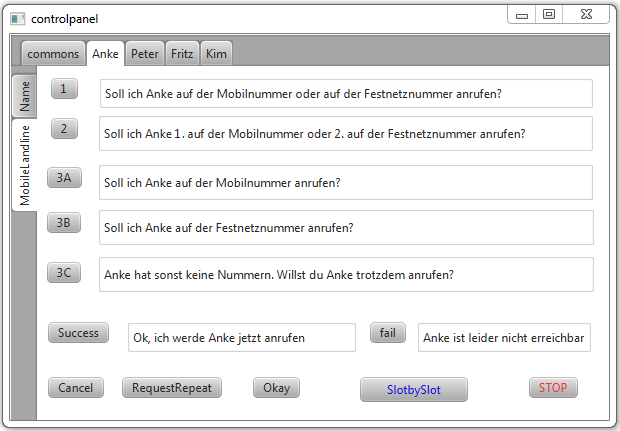
\includegraphics{controlpanel.png}
\caption{Controlpanel}
\label{cp1}
\end{figure}


\subsection{Versuchspersonen}

Hier wurden ebenfalls 12 Muttersprachler getestet. Davon waren fünf in der Altersgruppe 18-29, drei in der Altersgruppe 30-41 und vier in der Altergruppe 42-53. Drei haben Erfahrung mit Dialogsystemen, zwei spielen öfter Rennspiele und fünf fiel die Einführungsrunde einfach. Jede Versuchsperson wurde in eine Gruppe zugewiesen und hatte die selben Aufgabe wie in Verusch 1: 
\begin{enumerate}
\item Testrunde fahren
\item Fragebogen über Person ausfüllen (siehe \ref{fbperson1})
\item Strecke A fahren + Anke anrufen
\item Fragebogen über kognitive Belasung und letzten Dialog ausfüllen (siehe \ref{fbnasatlx1} und \ref{fbstrategien1} )
\item Strecke B fahren + Peter anrufen
\item Fragebogen über kognitive Belasung und letzten Dialog ausfüllen
\item Strecke C fahren + Fritz anrufen
\item Fragebogen über kognitive Belasung und letzten Dialog ausfüllen 
\item Kim anrufen
\item Fragebogen über kognitive Belasung und letzten Dialog ausfüllen 
\end{enumerate}

Wie in Versuch 1 sollten die Versuchspersonen ihre Eingabe deutlich über ein Tischmikrofon übermitteln und konnten sich die Personenprofile während des Dialoges auf einem Laptop ansehen.



\subsection{Auswertung}
Wie in Versuch 1 werden die Zeiten gemessen, die die Versuchsperson zum einen für das absolvieren der Strecke und zum anderen für das erfolgreiche Abschließen des Testszenarios benötigt (Unterkapitel \ref{messwerte}).
Nach jeder Rennrunde wird die Versuchsperson ebenfalls einen Fragebogen ausfüllen, welcher sich auf die subjektiv wahrgenommene kognitive Belastung und auf Merkmale der Disambiguierungsstrategien bezieht (Unterkapitel \ref{fragebogen}). Ebenfalls wird die Task Comlpletion ausgewertet und das Dialogverhalten untersucht. 
\subsubsection{gemessene Zeiten}
\label{messwerte}
\paragraph{Rennzeiten} 
~\\
%\textbf{Rennzeiten}\\

Die durchschnittlichen Rennzeiten für alle Strategien auf die einzelnen Strecken verteilt sind in Tabelle \ref{RZ3SV2} gelistet. 
\begin{longtable}{p{3cm}p{3cm}p{3cm}p{3cm} }
	\label{RZ3SV2}\\
	\caption[Durschnittszeiten Strategie pro Strecke]{Durschnittszeiten Strategie pro Strecke}\\
	\hline
	\textbf{Rennzeiten}&\textbf{Strategie 1}&\textbf{Strategie 2} &\textbf{Strategie 3}\\
	\hline
	\endfirsthead
	\hline
	\textbf{Rennzeiten}&\textbf{Strategie 1}&\textbf{Strategie 2} &\textbf{Strategie 3}\\
	\hline
	\endhead
Strecke A & 81 sek & 80,3 sek & 74,25 sek \\
Strecke B & 74,5 sek & 84,25 sek & 88 sek \\
Strecke C & 75 sek & 67,9 sek & 65 sek \\
\hline
\end{longtable}

Durch diese Ergebnisse kann man, wie in Versuch 1, keine Strategie bestimmen, mit der die Strecken am besten bzw. am schlechtesten gefahren wurden.
Dies könnte ebenfalls daran liegen, dass einzelne Werte durch schlechtere bzw. bessere Spieler in den Gruppen verfälscht wurden. Die Tabelle \ref{RennZeitenDis2} beinhaltet die durchschnittlichen Rennzeiten aller Strecken pro Strategie. 

\begin{longtable}{p{3cm}p{3cm}p{3cm}p{3cm} }
	\label{RennZeitenDis2}\\
	\caption[Durschnittszeiten pro Strategie]{Durschnittszeiten pro Strategie}\\
	\hline
	\textbf{Rennzeiten}&\textbf{Strategie 1}&\textbf{Strategie 2} &\textbf{Strategie 3}\\
	\hline
	\endfirsthead
	\hline
	\textbf{Rennzeiten}&\textbf{Strategie 1}&\textbf{Strategie 2} &\textbf{Strategie 3}\\
	\hline
	\endhead
Durschnitt & 76,83 sek & 77,47 sek & 76,73 sek \\
\hline
\end{longtable}
Der Unterschied in den Zeiten ist sehr gering und zudem ebenfalls statistisch nicht relevant. Diese Erkenntnis bekräftigt die in Versuch 1 getroffene Vermutung, dass die Rennzeit keinen Ausschluss darüber gibt, welche Strategie für die Autofahrt am geeignetsten ist. 

\paragraph{Dialogzeiten}
~\\
Neben den Zeiten für das Rennspiel werden auch die Dialogzeiten berechnet. 
Die Werte daraus werden wie in Verusch 1 dazu genutzt, um zu erforschen, mit welcher Strategie der kürzere Dialog möglich ist und um mögliche Unterschiede im Dialogverhalten zwischen einer hoch belastenden und eine weniger belastenden Versuchserperson zu erforschen. 
In Tabelle \ref{Durchschnittsdialogzeiten2} sind die Durchschnittswerte der Dialogzeiten aus Runde 1-3 einzeln und zusammen, sowie die Dialogzeiten aus Runde 4 festgehalten. 

\begin{longtable}{p{3cm}p{3cm}p{3cm}p{3cm} }
	\label{Durchschnittsdialogzeiten2}\\
	\caption[Durchschnittsdialogzeiten 2. Versuch]{Durchschnittsdialogzeiten 2. Versuch}\\
	\hline
	\textbf{Dialogzeiten}&\textbf{Strategie 1}&\textbf{Strategie 2} &\textbf{Strategie 3}\\
	\hline
	\endfirsthead
	\hline
	\textbf{Rennzeiten}&\textbf{Strategie 1}&\textbf{Strategie 2} &\textbf{Strategie 3}\\
	\hline
	\endhead
Strecke A & 25,76 sek & 38,32 sek & 33,98 sek \\
Strecke B & 31,41 sek & 40,2 sek & 36,61 sek \\
Strecke C  & 29,59 sek & 37,9 sek & 28,29 sek \\
\hline
\hline
Strecke A - C & 29,55 sek & 38,54 sek & 34,34 sek\\
\hline
ohne Strecke & 24,12 & 34,35 & 30,44 \\
\hline
\end{longtable}

Die zeitlichen Unterschiede der Disambiguierungsstrategien sind statistisch signifikant. An diesem Ergebnis sieht man, dass die erste Strategie den kürzesten Dialog ermöglichst und die zweite Strategie im Durchschnitt am längsten dauert. Dies gilt sowohl für die Runden mit Rennstrecke als auch für die Runden ohne Rennspiel. Der Vergleich der letzten beiden Reihen macht deutlich, dass auch in diesem Verusch der Dialog ohne Rennspiel im Durchschnitt deutlich kürzer war, als der Dialog mit Rennspiel. Wie in Versuch 1 kommt man hier zu der Vermutung, dass die Reaktionszeit bei geringer Belastung kleiner ist, als bei höherer Belastung.  

\subsubsection{Fragebogen}
\label{fragebogen}
Zu Beginn des Versuch wird mit dem selben Fragebogen wie in Versuch 1 Informationen über die Versuchsperson abgefragt. Nach jeder Runde wird ebenefalls der gleiche Fragebogen wie im ersten Versuch ausgefüllt, bestehend aus einem Teil des NASA-TLX Tests und einem Teil über die zuletzt gehörte Strategie.

\paragraph{Nasa-TLX}
~\\
Dieser Teil des Fragebogens wird wie im ersten Versuch dazu genutzt um zu erforschen, bei welcher Strategie eine höhere Belastung empfunden wurde und ob es Unterschiede in der empfundenen Belastung in den Runden mit Rennspiel und ohne Rennspiel gibt. 
Die nachfolgender Tabelle zeigt die Ergebnisse jeder Frage pro Strategie.
\begin{longtable}{|p{4cm}|p{2cm}|p{2cm}|p{2cm}|p{2cm}|}
	\hline
		\textbf{Antwortenintervall}&\textbf{Strategien}&\multicolumn{3}{c|}{\textbf{Ergebnisse bestimmter Runden}}\\
	&&\textbf{1-4}&\textbf{1-3} &\textbf{4}\\
	\hline
	\endfirsthead
	\hline
	\textbf{Antwortenintervall}&\textbf{Strategien}&\textbf{Runden 1-4}&\textbf{Runden 1-3} &\textbf{Runde 4}\\
	\hline
	\endhead
		\multicolumn{5}{l}{\textbf{Geistige Anforderung}}\\
		\hline
\multirow{3}{4cm}{1: gering \newline 6: hoch} & Strategie 1 &  2,31 & 2,67 & 1,25 \\
 & Strategie 2 & 2,31 & 2,58 & 1,5\\
 & Strategie 3 & 2,56 & 2,83 & 1,75 \\
\hline
		\multicolumn{5}{l}{\textbf{Körperliche Anforderung}}\\
		\hline
\multirow{3}{4cm}{1: gering \newline 6: hoch} & Strategie 1 & 1,67 & 2,17 & 1 \\
 & Strategie 2 & 2,06 & 2,25 & 1,5 \\
 & Strategie 3 & 1,94 & 2,08 & 1,5 \\
\hline
		\multicolumn{5}{l}{\textbf{Zeitliche Anforderung}}\\
		\hline
\multirow{3}{4cm}{1: gering \newline 6: hoch} & Strategie 1 & 2 & 2,25 & 1,25 \\
 & Strategie 2 & 2,25 & 2,5 & 1,5 \\
 & Strategie 3 & 1,94 & 2,17 & 1,25 \\
\hline
		\multicolumn{5}{l}{\textbf{Leistung}}\\
		\hline
\multirow{3}{4cm}{1: gering \newline 6: hoch} & Strategie 1 & 5,13 & 4,83 & 6 \\
 & Strategie 2 & 4,88 & 4,67 & 5,5 \\
 & Strategie 3 & 4,56 & 4,08 & 6 \\
\hline
		\multicolumn{5}{l}{\textbf{Anstrengung}}\\
		\hline
\multirow{3}{4cm}{1: gering \newline 6: hoch} & Strategie 1 & 2,38 & 2,83 & 1 \\
 & Strategie 2 & 2,44 & 2,67 & 1,75 \\
 & Strategie 3 & 2,31 & 2,67 & 1,25\\
\hline
		\multicolumn{5}{l}{\textbf{Frustration}}\\
		\hline
\multirow{3}{4cm}{1: gering \newline 6: hoch} & Strategie 1 & 1,94 & 2,25 & 1 \\
 & Strategie 2 & 1,94 & 2 & 1,75 \\
 & Strategie 3 & 2,31 & 2,58 & 1,5 \\
\hline
\end{longtable}

Auch in diesem Versuch sind die Antworten der einzelnen Strategien nicht signifikant und es ist kein eindeutiges Muster zu erkennen, welche Strategie am unbelastendsten ist. Beim Vergleich der Antworten von Runde 1-3 mit Runde 4 wird jedoch deutlich, dass bei allen Fragen die Runde mit Rennspiel als belastender gewertet wurde als die Runde ohne Rennspiel. Dieses Ergebnis bestätigt dass Ergebnis aus Versuch 1 und bestärkt die Aussage, dass hier ein Unterschied in der Belastung empfunden worder ist.  

\paragraph{Strategien}
~\\
\begin{longtable}{|p{4cm}|p{2cm}|p{2cm}|p{2cm}|p{2cm}|}
	\hline
		\textbf{Antwortenintervall}&\textbf{Strategien}&\multicolumn{3}{c|}{\textbf{Ergebnisse bestimmter Runden}}\\
	&&\textbf{1-4}&\textbf{1-3} &\textbf{4}\\
	\hline
	\endfirsthead
	\hline
	\textbf{Antwortenintervall}&\textbf{Strategien}&\textbf{Runden 1-4}&\textbf{Runden 1-3} &\textbf{Runde 4}\\
	\hline
	\endhead
		\multicolumn{5}{l}{\textbf{Der Dialog lenkte mich vom Rennspiel ab}}\\
		\hline
\multirow{3}{4cm}{1: kaum \newline 6: stark} & Strategie 1 & \multirow{3}{2,5cm}{in Runde 4 nicht beantwortet} & 3,5  & \multirow{3}{2,5cm}{nicht beantwortet} \\
 & Strategie 2 & & 2,92 & \\
 & Strategie 3 & & 3,17 & \\
\hline
		\multicolumn{5}{l}{\textbf{Die Nachfragen erleichterten es mir, den Anruf korrekt aufzubauen}}\\
		\hline
\multirow{3}{4cm}{1: erleichterte es\newline  6: erschwerte es} & Strategie 1 & 2,44 & 2,58 & 2 \\
 & Strategie 2 & 2,25 & 2,33 & 2 \\
 & Strategie 3 & 2,38 & 2,5 & 2 \\
\hline
		\multicolumn{5}{l}{\textbf{Wussten Sie, wann das System Spracheingaben erwartete?}}\\
		\hline
\multirow{3}{4cm}{1: immer \newline  6: nicht immer} & Strategie 1 & 1,63 & 1,67 & 1,5 \\
 & Strategie 2 & 1,5 & 1,5 & 1,5 \\
 & Strategie 3 & 1,57 & 1,5 & 1,75 \\
\hline
		\multicolumn{5}{l}{\textbf{Wie gefiel Ihnen der Dialog insgesamt?}}\\
		\hline
\multirow{3}{4cm}{1: sehr gut \newline  6: weniger gut} & Strategie 1 & 2,94 & 2,83 & 3,25 \\
 & Strategie 2 & 2,44 & 2,42 & 2,5 \\
 & Strategie 3 & 2,38 & 2,3 & 2,5 \\
\hline
		\multicolumn{5}{l}{\textbf{Fiel es Ihnen einfacher, den Dialog ohne Rennspiel zu führen?}}\\
		\hline
\multirow{3}{4cm}{1: viel einfacher \newline  6: nicht einfacher} & Strategie 1 & \multirow{3}{2,5cm}{in Runden 1-3 nicht beantwortet} & \multirow{3}{2,5cm}{nicht beantwortet} & 2,75 \\
 & Strategie 2 & & & 3 \\
 & Strategie 3 & & & 2,5\\
\hline
		\multicolumn{5}{l}{\textbf{Welcher Anruf gefiel Ihnen insgesamt am besten?}}\\
		\hline
\multirow{3}{4cm}{Anruf bzw. Strategie auswählbar} & Strategie 1 & 16,7\% & & \\
 & Strategie 2 & 33,3\% && \\
 & Strategie 3 & 50\% && \\
\hline
\end{longtable}

Im Gegensatz zum ersten Verusch kann man durch die ersten vier Fragen keine Strategie erkennen, die eindeutig am besten bewertet wurde. Die vierte Frage, welche den Dialog insgesamt bewertet lies, stimmt jedoch mit dem Ergebnis der letzten Frage überein. Der Dialog mit Strategie 3 wurde in Frage vier am besten bewertet und auch am häufigsten als Favorit in der letzten Frage gewählt. Parallel gilt dies für Strategie 1, welche am schlechtesten bewertet wurde und auch am seltensten bei der letzten Frage gewählt wurde. Die vorletzte Frage zeigt auch in diesem Versuch, dass es leichter fiel, den Dialog ohne Rennspiel zu führen und bestätigt damit das Ergebnis des Nasa-TLX-Tests.

\subsubsection{Task Completion}
Für jede Strategie wird ebenfalls die Task Completion ausgewertet, welche besagt, mit welchem Erfolg der Anruf ausgeführt wurde. Folgenden Punktzahlen sind für jede Strategie möglich:
\begin{itemize}
\item 0 Punkte, wenn kein Slot richtig gefüllt wird
\item 1 Punkt, wenn ein Slot richtig gefüllt wird
\item 2 Punkte, wenn alle Slots richtig gefüllt wird
\end{itemize}
Zur Auswertung wird dann pro Strategie eine Durschnittspunktzahl berechnet, welche in \ref{TCV2} stehen. 

\begin{longtable}{p{3cm}p{3cm}p{3cm}p{3cm} }
	\label{TCV2}\\
	\caption[Task Completion Versuch 2]{Task Completion Versuch 2}\\
	\hline
\textbf{Strategien}&\textbf{insgesamt}&\textbf{Runde 1-3} &\textbf{Runde 4}\\
	\hline
	\endfirsthead
	\hline
	\textbf{Strategien}&\textbf{\O TC insgesamt}&\textbf{\O TC Runde 1-3} &\textbf{\O TC Runde 4}\\
	\hline
	\endhead
1. Strategie & 1,88 & 1,83 & 2  \\
2. Strategie & 1,81 & 1,75 & 2  \\
3. Strategie & 1,56 & 1,42 & 2  \\
\hline
Insgesamt & & 1,67 & 2 \\ 
\hline
\end{longtable}

Hier zeigt sich klar, dass die Dialoge in Runde 4 ohne Fehler erfolgten und somit im Durchschnitt erfolgreicher waren als die Runden mit Rennspiel. Es fällt auf, dass die Strategie, die in diesem Versuch als am beliebtesten ausgewertet wurde am meisten Fehler aufweist. Dabei kommt erneut die Frage aus Versuch 1 auf, ob man hier eine Verbindung ziehen kann und ob die Versuchspersonen bemerkten, dass sie die Slots falsch gefüllt haben. 
Grundsätzlich kann man aus diesem Ergebnis sehen, dass insgesamt der Anruf am häufigsten korrekt mit Strategie 1 und am seltensten korrekt mit Strategie 2 ausgeführt werden konnte. 

\subsubsection{Dialoverhalten}
In diesem Versuch wurden mit den selben Antwortmöglichkeiten geantwortet wie in Versuch 1 (siehe Tabelle \ref{Dialogverhalten11}.

Die Häufigkeit dieser Antworten pro Stratgie aus Runde 1-3 sind in nachfolgender Tabelle aufgelistet.

\begin{longtable}{p{3cm}p{3cm}p{3cm}p{3cm} }
	\label{Dialogverhalten12}\\
	\caption[Antwortenverteilung pro Strategie]{Antwortenverteilung pro Strategie}\\
	\hline
\textbf{Antwort-möglichkeiten}&\textbf{Strategie 1}&\textbf{Strategie 2} &\textbf{Strategie 3}\\
	\hline
	\endfirsthead
	\hline
	\textbf{Antwortmöglichkeiten}&\textbf{Strategie 1}&\textbf{Strategie 2} &\textbf{Strategie 3}\\
	\hline
	\endhead
Slots & 100\% & 62,5\%\ & 0\%  \\
Position & 0\% & 37,5\% & 0\%  \\
ja/nein & 0\% & 0\%  & 100 \%  \\
\hline
\end{longtable}
Diese Ergebnisse sind mit denen aus Versuch 1 zu vergleichen. 
Außerdem stimmen hier ebenfalls die Antwortmöglichkeiten bei hoher Belastung mit denen bei niedrigen Belastung überein, weshalb kein Unterschied im Dialogverhalten bei unterschiedlicher Belastung erkennbar ist. 




\subsection{Resultat}
Aus den Resultaten aus Kapitel \ref{auswertung1} wird die effizienteste Strategie ermittelt. \newline

Durch die Dialogzeiten wird klar, dass Strategie 1 sowohl in den Runde mit als auch ohne Rennspiel den kürzesten Dialog ermöglicht. Aus den Antworten des Nasa-TLX Teil des Fragebogens wird deutlich, dass Strategie 1 von den Benutzern am wenigsten belastend gewertet wurde.  In allen Fragen des zweiten Teil des Fragebogens wurde ebenfalls Strategie 1 am besten bewertet und durch die letzten Frage deutlich als beliebteste Strategie gewertet. Laut Task Completion ist Strategie 2 auf allen Runden am erfolgreichsten, Strategie 1 und 2 in den Runden mit Rennstrecke jedoch gleich gut.
Durch diese Erkenntnisse kommt man klar zu dem Entschluss, das Strategie 1 eindeutig die beliebteste und effizienteste Strategie ist. \newline \newline
Da dieses Resultat bereits nach wenigen Versuchspersonen zu erwarten war und die Frage aufkam, ob die erste Strategie auch bei einer längeren Disambiguierung am geeignetsten ist, hat man den Versuch bereits nach 12 Versuchspersonen abgebrochen und einen zweiten Versuch gestartet. Der zweite Versuch ist identisch mit dem ersten Versuch, unterscheidet sich jedoch in der Anzahl der in der Disambiguierung vorgeschlagenen Slotfüller.
\begin{comment}
\subsubsection{Zeiten}
\paragraph{Rennzeiten}
~\\
\begin{longtable}{p{3cm}p{3cm}p{3cm}p{3cm} }
	\label{durchschnittsvorl}\\
	\caption[Durschnittszeiten Strategie pro Strecke]{Durschnittszeiten Strategie pro Strecke}\\
	\hline
	\textbf{Rennzeiten}&\textbf{Strategie 1}&\textbf{Strategie 2} &\textbf{Strategie 3}\\
	\hline
	\endfirsthead
	\hline
	\textbf{Rennzeiten}&\textbf{Strategie 1}&\textbf{Strategie 2} &\textbf{Strategie 3}\\
	\hline
	\endhead
Strecke A & 81 sek & 80,3 sek & 74,25 sek \\
Strecke B & 74,5 sek & 84,25 sek & 88 sek \\
Strecke C & 75 sek & 67,9 sek & 65 sek \\
\hline
Strecke A - C & 76,83 & 77,47 & 76,73 \\
\hline
\end{longtable}

\paragraph{Dialogzeiten}
~\\

\begin{longtable}{p{3cm}p{3cm}p{3cm}p{3cm} }
	\label{durchschnittsvorl}\\
	\caption[Durchschnittszeiten Strategie pro Strecke]{Durschnittszeiten Strategie pro Strecke}\\
	\hline
	\textbf{Dialogzeiten}&\textbf{Strategie 1}&\textbf{Strategie 2} &\textbf{Strategie 3}\\
	\hline
	\endfirsthead
	\hline
	\textbf{Rennzeiten}&\textbf{Strategie 1}&\textbf{Strategie 2} &\textbf{Strategie 3}\\
	\hline
	\endhead
Strecke A & 25,76 sek & 38,32 sek & 33,98 sek \\
Strecke B & 31,41 sek & 40,2 sek & 36,61 sek \\
Strecke C  & 29,59 sek & 37,9 sek & 28,29 sek \\
\hline
\hline
Strecke A - C & 29,55 sek & 38,54 sek & 34,34 sek\\
\hline
ohne Strecke & 24,12 & 34,35 & 30,44 \\
\hline
\end{longtable}
 
\begin{longtable}{p{4cm}p{4cm}p{4cm}}
	\label{Dialogzeiten13vs4}\\
	\caption[Durschnittszeiten mit Rennspiel versus ohne Rennspiel]{Durschnittszeiten mit Rennspiel versus ohne Rennspiel}\\
	\hline
	\textbf{Dialogzeiten}&\textbf{Runde 1-3}&\textbf{Runde 4}\\
	\hline
	\endfirsthead
	\hline
	\textbf{Dialogzeiten}&\textbf{Runde 1-3}&\textbf{Runde 4}\\
	\hline
	\endhead
Durschnitt &  34,64 sek & 29,63 sek \\


\hline
\end{longtable}

\subsubsection{Fragebogen}
\paragraph{Nasa-TLX}
~\\
\begin{longtable}{|p{4cm}|p{2cm}|p{2cm}|p{2cm}|p{2cm}|}
	\hline
		\textbf{Antwortenintervall}&\textbf{Strategien}&\multicolumn{3}{c|}{\textbf{Ergebnisse bestimmter Runden}}\\
	&&\textbf{1-4}&\textbf{1-3} &\textbf{4}\\
	\hline
	\endfirsthead
	\hline
	\textbf{Antwortenintervall}&\textbf{Strategien}&\textbf{Runden 1-4}&\textbf{Runden 1-3} &\textbf{Runde 4}\\
	\hline
	\endhead
		\multicolumn{5}{l}{\textbf{Geistige Anforderung}}\\
		\hline
\multirow{3}{4cm}{1: gering \newline 6: hoch} & Strategie 1 &  2,31 & 2,67 & 1,25 \\
 & Strategie 2 & 2,31 & 2,58 & 1,5\\
 & Strategie 3 & 2,56 & 2,83 & 1,75 \\
\hline
		\multicolumn{5}{l}{\textbf{Körperliche Anforderung}}\\
		\hline
\multirow{3}{4cm}{1: gering \newline 6: hoch} & Strategie 1 & 1,67 & 2,17 & 1 \\
 & Strategie 2 & 2,06 & 2,25 & 1,5 \\
 & Strategie 3 & 1,94 & 2,08 & 1,5 \\
\hline
		\multicolumn{5}{l}{\textbf{Zeitliche Anforderung}}\\
		\hline
\multirow{3}{4cm}{1: gering \newline 6: hoch} & Strategie 1 & 2 & 2,25 & 1,25 \\
 & Strategie 2 & 2,25 & 2,5 & 1,5 \\
 & Strategie 3 & 1,94 & 2,17 & 1,25 \\
\hline
		\multicolumn{5}{l}{\textbf{Leistung}}\\
		\hline
\multirow{3}{4cm}{1: gering \newline 6: hoch} & Strategie 1 & 5,13 & 4,83 & 6 \\
 & Strategie 2 & 4,88 & 4,67 & 5,5 \\
 & Strategie 3 & 4,56 & 4,08 & 6 \\
\hline
		\multicolumn{5}{l}{\textbf{Anstrengung}}\\
		\hline
\multirow{3}{4cm}{1: gering \newline 6: hoch} & Strategie 1 & 2,38 & 2,83 & 1 \\
 & Strategie 2 & 2,44 & 2,67 & 1,75 \\
 & Strategie 3 & 2,31 & 2,67 & 1,25\\
\hline
		\multicolumn{5}{l}{\textbf{Frustration}}\\
		\hline
\multirow{3}{4cm}{1: gering \newline 6: hoch} & Strategie 1 & 1,94 & 2,25 & 1 \\
 & Strategie 2 & 1,94 & 2 & 1,75 \\
 & Strategie 3 & 2,31 & 2,58 & 1,5 \\
\hline
\end{longtable}


\paragraph{Strategien}
~\\
\begin{longtable}{|p{4cm}|p{2cm}|p{2cm}|p{2cm}|p{2cm}|}
	\hline
		\textbf{Antwortenintervall}&\textbf{Strategien}&\multicolumn{3}{c|}{\textbf{Ergebnisse bestimmter Runden}}\\
	&&\textbf{1-4}&\textbf{1-3} &\textbf{4}\\
	\hline
	\endfirsthead
	\hline
	\textbf{Antwortenintervall}&\textbf{Strategien}&\textbf{Runden 1-4}&\textbf{Runden 1-3} &\textbf{Runde 4}\\
	\hline
	\endhead
		\multicolumn{5}{l}{\textbf{Der Dialog lenkte mich vom Rennspiel ab}}\\
		\hline
\multirow{3}{4cm}{1: kaum \newline 6: stark} & Strategie 1 & \multirow{3}{2,5cm}{in Runde 4 nicht beantwortet} & 3,5  & \multirow{3}{2,5cm}{nicht beantwortet} \\
 & Strategie 2 & & 2,92 & \\
 & Strategie 3 & & 3,17 & \\
\hline
		\multicolumn{5}{l}{\textbf{Die Nachfragen erleichterten es mir, den Anruf korrekt aufzubauen}}\\
		\hline
\multirow{3}{4cm}{1: erleichterte es\newline  6: erschwerte es} & Strategie 1 & 2,44 & 2,58 & 2 \\
 & Strategie 2 & 2,25 & 2,33 & 2 \\
 & Strategie 3 & 2,38 & 2,5 & 2 \\
\hline
		\multicolumn{5}{l}{\textbf{Wussten Sie, wann das System Spracheingaben erwartete?}}\\
		\hline
\multirow{3}{4cm}{1: immer \newline  6: nicht immer} & Strategie 1 & 1,63 & 1,67 & 1,5 \\
 & Strategie 2 & 1,5 & 1,5 & 1,5 \\
 & Strategie 3 & 1,57 & 1,5 & 1,75 \\
\hline
		\multicolumn{5}{l}{\textbf{Wie gefiel Ihnen der Dialog insgesamt?}}\\
		\hline
\multirow{3}{4cm}{1: sehr gut \newline  6: weniger gut} & Strategie 1 & 2,94 & 2,83 & 3,25 \\
 & Strategie 2 & 2,44 & 2,42 & 2,5 \\
 & Strategie 3 & 2,38 & 2,3 & 2,5 \\
\hline
		\multicolumn{5}{l}{\textbf{Fiel es Ihnen einfacher, den Dialog ohne Rennspiel zu führen?}}\\
		\hline
\multirow{3}{4cm}{1: viel einfacher \newline  6: nicht einfacher} & Strategie 1 & \multirow{3}{2,5cm}{in Runden 1-3 nicht beantwortet} & \multirow{3}{2,5cm}{nicht beantwortet} & 2,75 \\
 & Strategie 2 & & & 3 \\
 & Strategie 3 & & & 2,5\\
\hline
		\multicolumn{5}{l}{\textbf{Welcher Anruf gefiel Ihnen insgesamt am besten?}}\\
		\hline
\multirow{3}{4cm}{Anruf bzw. Strategie auswählbar} & Strategie 1 & 16,7\% & & \\
 & Strategie 2 & 33,3\% && \\
 & Strategie 3 & 50\% && \\
\hline
\end{longtable}
\subsubsection{Task Completion}
\begin{longtable}{p{3cm}p{3cm}p{3cm}p{3cm} }
	\label{Dialogzeiten}\\
	\caption[Durschnittliche Task Completion (TC)]{Durschnittliche Task Completion (TC)}\\
	\hline
\textbf{Strategien}&\textbf{insgesamt}&\textbf{Runde 1-3} &\textbf{Runde 4}\\
	\hline
	\endfirsthead
	\hline
	\textbf{Strategien}&\textbf{\O TC insgesamt}&\textbf{\O TC Runde 1-3} &\textbf{\O TC Runde 4}\\
	\hline
	\endhead
1. Strategie & 1,88 & 1,83 & 2  \\
2. Strategie & 1,81 & 1,75 & 2  \\
3. Strategie & 1,56 & 1,42 & 2  \\
\hline
Insgesamt & & 1,67 & 2 \\ 
\hline
\end{longtable}
Fragebogen: NASA-TLX\\
Wurde der Task zu ende geführt?\\
Wurde dem User klar, welche Eingaben er machen konnte (das erste, der zweite..)\\
Wurde richtig geantwortet?\\
Konkrete Zahlen besser als Benutzermeinung \\
wie einig sind sich die Benutzer\\
Extreme vorhanden?\\
wie kann man auswerten?
\begin{itemize}
\item Reaktionszeit
\item Taskdauer
\item Reaktion während Vorlesens bewerten
\item vergleich zeit mit und ohne CL
\item Interaktion bewerten lassen (skala 1-10)
 \begin{itemize}
\item Wie intuitiv 
\item angnehm?
\item ablenkend oder störend während der Fahrt?
\item wie aufmerksam musste man sein 

\end{itemize}
\end{itemize}

\end{comment}


\section{Ergebnisse}
\label{Ergebnisse}

\subsection{Rennzeiten}
\subsection{Dialogzeiten}
\subsection{Fragebogen}
\subsection{Task Completion}
\subsection{Dialogverhalten}

\section{Diskussion}
\label{discussion}
was habe ich gemacht\\
wie waren die überlegungen\\
warum wurden welche Entscheidungen getroffen\\
warum wurden andere verworfen\\
Rennspielzeiten uncool\\
Task Completion in real besser, da VP nciht dumm\\
\subsection{Allgemeine Diskussion}
Warum kann das Ergebnis verallgemeinert werden (cognitive load)\\
gilt nicht nur für Rennspielsimulation, sondern auch für andere Interaktionen(?)
\subsection{Vergleichbare Studien}
Vergleich mit anderen Studien möglich?\\
\subsection{Future Work}
VP in Gruppen unterteilen (je nach Wissenstand)\\
VP in Gruppen mit unterschiedlichen DisStrat aufteilen\\
andere DisSrat.\\
Unterschiede VP versch. Alters\\


\section{Schlusswort}




\newpage
\appendix
\pagenumbering{roman}

%\section{Referenzen}

%\bibliographystyle{geralpha}
%\bibliography{meinbib}

\begin{thebibliography}{Maron \& Ames, 1982}

	\bibitem[Ang et al., 2006]{CLmmorpg} Chee Siang Ang, Panayiotis Zaphiris, Shumalai Mahmood: \textit{Cognitive Load Issues in MMORPGs} 
(2006).

	\bibitem[Minker et al., 2002]{idsia} W. Minker, U. Haiber, P. Heisterkamp, S. 
Scheible: \textit{intelligent dialog strategy for accesssing infotainment applications in mobile 
environments} ISCA Tutorial and Research Workshop (ITRW) on Multi-Modal Dialogue in Mobile 
Environments, Irsee (Germany) (June 2002).

\bibitem[Mishra et al., 2004]{Wozhcd} R Mishra, E Shriberg, S Upson, J Chen, F Weng, S Peters,
L Cavedon, J Niekrasz, H Cheng, and H Bratt. \textit{A wizard of Oz framework for collecting spoken human-computer dialogs.} (2004)

	\bibitem[Tsiakoulis et al, 2012]{eCLDS} P. Tsiakoulis, M. Henderson, B. Thomson, K. Yu, E. Tzirkel, S. Young: \textit{The Effect of Cognitive Load on a Statistical Dialogue System} Proceedings of the 13th Annual Meeting of the Special Interest Group on Discourse and Dialogue (SIGDIAL), pages 74–78,
Seoul, South Korea, (July 2012).

\bibitem [Villing, 2009]{DbCL} Jessica Villing: \textit{Dialogue behaviour under high cognitive load} Proceedings of SIGDIAL 2009: the 10th Annual Meeting of the Special Interest Group in Discourse and Dialogue, pages 322–325,(2009)



\bibitem[Yin et al., 2007]{AclD} Bo Yin, Natalie Ruiz, Fang Chen, M. Asif Khawaja: \textit{Automatic cognitive load detection from speech feature} in OZCHI ’07: Proceedings of the 19th Australasian conference on Computer-Human Interaction 249-255. 



\end{thebibliography}


\end{document}
